\documentclass[a4paper,12pt,twoside]{memoir}

% Castellano
\usepackage[spanish,es-tabla]{babel}
\selectlanguage{spanish}
\usepackage[utf8]{inputenc}
\usepackage[T1]{fontenc}
\usepackage{lmodern} % Scalable font
\usepackage{microtype}
\usepackage{placeins}


\RequirePackage{booktabs}
\RequirePackage[table]{xcolor}
\RequirePackage{xtab}
\RequirePackage{multirow}

\usepackage{pdfpages}

% Links
\usepackage[colorlinks]{hyperref}
\hypersetup{
	allcolors = {red}
}

% Ecuaciones
\usepackage{amsmath}
\usepackage{amssymb}

\newcommand{\hubu}{\hline \rule{0pt}{2.7ex}}
\usepackage{eurosym} % para el euro

% Rutas de fichero / paquete
\newcommand{\ruta}[1]{{\sffamily #1}}

% Párrafos
\nonzeroparskip


% Imagenes
\usepackage{graphicx}
\newcommand{\imagen}[2]{
	\begin{figure}[!h]
		\centering
		\includegraphics[width=0.9\textwidth]{#1}
		\caption{#2}\label{fig:#1}
	\end{figure}
	\FloatBarrier
}

\newcommand{\imagenflotante}[2]{
	\begin{figure}%[!h]
		\centering
		\includegraphics[width=0.9\textwidth]{#1}
		\caption{#2}\label{fig:#1}
	\end{figure}
}



% El comando \figura nos permite insertar figuras comodamente, y utilizando
% siempre el mismo formato. Los parametros son:
% 1 -> Porcentaje del ancho de página que ocupará la figura (de 0 a 1)
% 2 --> Fichero de la imagen
% 3 --> Texto a pie de imagen
% 4 --> Etiqueta (label) para referencias
% 5 --> Opciones que queramos pasarle al \includegraphics
% 6 --> Opciones de posicionamiento a pasarle a \begin{figure}
\newcommand{\figuraConPosicion}[6]{%
  \setlength{\anchoFloat}{#1\textwidth}%
  \addtolength{\anchoFloat}{-4\fboxsep}%
  \setlength{\anchoFigura}{\anchoFloat}%
  \begin{figure}[#6]
    \begin{center}%
      \Ovalbox{%
        \begin{minipage}{\anchoFloat}%
          \begin{center}%
            \includegraphics[width=\anchoFigura,#5]{#2}%
            \caption{#3}%
            \label{#4}%
          \end{center}%
        \end{minipage}
      }%
    \end{center}%
  \end{figure}%
}

%
% Comando para incluir imágenes en formato apaisado (sin marco).
\newcommand{\figuraApaisadaSinMarco}[5]{%
  \begin{figure}%
    \begin{center}%
    \includegraphics[angle=90,height=#1\textheight,#5]{#2}%
    \caption{#3}%
    \label{#4}%
    \end{center}%
  \end{figure}%
}
% Para las tablas
\newcommand{\otoprule}{\midrule [\heavyrulewidth]}
%
% Nuevo comando para tablas pequeñas (menos de una página).
\newcommand{\tablaSmall}[5]{%
 \begin{table}
  \begin{center}
   \rowcolors {2}{gray!35}{}
   \begin{tabular}{#2}
    \toprule
    #4
    \otoprule
    #5
    \bottomrule
   \end{tabular}
   \caption{#1}
   \label{tabla:#3}
  \end{center}
 \end{table}
}

%
% Nuevo comando para tablas pequeñas (menos de una página).
\newcommand{\tablaSmallSinColores}[5]{%
 \begin{table}[H]
  \begin{center}
   \begin{tabular}{#2}
    \toprule
    #4
    \otoprule
    #5
    \bottomrule
   \end{tabular}
   \caption{#1}
   \label{tabla:#3}
  \end{center}
 \end{table}
}

\newcommand{\tablaApaisadaSmall}[5]{%
\begin{landscape}
  \begin{table}
   \begin{center}
    \rowcolors {2}{gray!35}{}
    \begin{tabular}{#2}
     \toprule
     #4
     \otoprule
     #5
     \bottomrule
    \end{tabular}
    \caption{#1}
    \label{tabla:#3}
   \end{center}
  \end{table}
\end{landscape}
}

%
% Nuevo comando para tablas grandes con cabecera y filas alternas coloreadas en gris.
\newcommand{\tabla}[6]{%
  \begin{center}
    \tablefirsthead{
      \toprule
      #5
      \otoprule
    }
    \tablehead{
      \multicolumn{#3}{l}{\small\sl continúa desde la página anterior}\\
      \toprule
      #5
      \otoprule
    }
    \tabletail{
      \hline
      \multicolumn{#3}{r}{\small\sl continúa en la página siguiente}\\
    }
    \tablelasttail{
      \hline
    }
    \bottomcaption{#1}
    \rowcolors {2}{gray!35}{}
    \begin{xtabular}{#2}
      #6
      \bottomrule
    \end{xtabular}
    \label{tabla:#4}
  \end{center}
}

%
% Nuevo comando para tablas grandes con cabecera.
\newcommand{\tablaSinColores}[6]{%
  \begin{center}
    \tablefirsthead{
      \toprule
      #5
      \otoprule
    }
    \tablehead{
      \multicolumn{#3}{l}{\small\sl continúa desde la página anterior}\\
      \toprule
      #5
      \otoprule
    }
    \tabletail{
      \hline
      \multicolumn{#3}{r}{\small\sl continúa en la página siguiente}\\
    }
    \tablelasttail{
      \hline
    }
    \bottomcaption{#1}
    \begin{xtabular}{#2}
      #6
      \bottomrule
    \end{xtabular}
    \label{tabla:#4}
  \end{center}
}

%
% Nuevo comando para tablas grandes sin cabecera.
\newcommand{\tablaSinCabecera}[5]{%
  \begin{center}
    \tablefirsthead{
      \toprule
    }
    \tablehead{
      \multicolumn{#3}{l}{\small\sl continúa desde la página anterior}\\
      \hline
    }
    \tabletail{
      \hline
      \multicolumn{#3}{r}{\small\sl continúa en la página siguiente}\\
    }
    \tablelasttail{
      \hline
    }
    \bottomcaption{#1}
  \begin{xtabular}{#2}
    #5
   \bottomrule
  \end{xtabular}
  \label{tabla:#4}
  \end{center}
}



\definecolor{cgoLight}{HTML}{EEEEEE}
\definecolor{cgoExtralight}{HTML}{FFFFFF}

%
% Nuevo comando para tablas grandes sin cabecera.
\newcommand{\tablaSinCabeceraConBandas}[5]{%
  \begin{center}
    \tablefirsthead{
      \toprule
    }
    \tablehead{
      \multicolumn{#3}{l}{\small\sl continúa desde la página anterior}\\
      \hline
    }
    \tabletail{
      \hline
      \multicolumn{#3}{r}{\small\sl continúa en la página siguiente}\\
    }
    \tablelasttail{
      \hline
    }
    \bottomcaption{#1}
    \rowcolors[]{1}{cgoExtralight}{cgoLight}

  \begin{xtabular}{#2}
    #5
   \bottomrule
  \end{xtabular}
  \label{tabla:#4}
  \end{center}
}


\graphicspath{ {./img/} }

% Capítulos
\chapterstyle{bianchi}
\newcommand{\capitulo}[2]{
	\setcounter{chapter}{#1}
	\setcounter{section}{0}
	\chapter*{#2}
	\addcontentsline{toc}{chapter}{#1. #2}
	\markboth{#2}{#2}
}

% Apéndices
\renewcommand{\appendixname}{Apéndice}
\renewcommand*\cftappendixname{\appendixname}

\newcommand{\apendice}[1]{
	%\renewcommand{\thechapter}{A}
	\chapter{#1}
}

\renewcommand*\cftappendixname{\appendixname\ }

% Formato de portada
\makeatletter
\usepackage{xcolor}
\newcommand{\tutor}[1]{\def\@tutor{#1}}
\newcommand{\course}[1]{\def\@course{#1}}
\definecolor{cpardoBox}{HTML}{E6E6FF}
\def\maketitle{
  \null
  \thispagestyle{empty}
  % Cabecera ----------------
\begin{center}%
	{\noindent\Huge Universidades de Burgos, León y Valladolid}\vspace{.5cm}%
	
	{\noindent\Large Máster universitario}\vspace{.5cm}%
	
	{\noindent\Huge \textbf{Inteligencia de Negocio y Big~Data en Entornos Seguros}}\vspace{.5cm}%
\end{center}%

\begin{center}%
	
\includegraphics[height=3cm]{img/escudoUBU} \hspace{1cm}
	
\includegraphics[height=3cm]{img/escudoUVA} \hspace{1cm}
	
\includegraphics[height=3cm]{img/escudoULE} \vspace{1cm}%
\end{center}%

  \vfill
  % Título proyecto y escudo informática ----------------
  \colorbox{cpardoBox}{%
    \begin{minipage}{.9\textwidth}
      \vspace{.2cm}\Large
      \begin{center}
      \textbf{Trabajo Fin de Máster}\vspace{.6cm}\\
      \textbf{\LARGE\@title{}}
      \end{center}
      \vspace{.2cm}
    \end{minipage}

  }%
  
  \vfill
  % Datos de alumno, curso y tutores ------------------
  \begin{center}%
  {%
    \noindent\LARGE
    Presentado por \@author{}\\ 
    en Universidad de Burgos --- \@date{}\\
    Tutor: \@tutor{}\\
  }%
  \end{center}%
  \null
  \cleardoublepage
  }
\makeatother

\usepackage{subcaption}


% Default fixed font does not support bold face
\DeclareFixedFont{\ttb}{T1}{txtt}{bx}{n}{12} % for bold
\DeclareFixedFont{\ttm}{T1}{txtt}{m}{n}{12}  % for normal

% Custom colors
\usepackage{color}
\definecolor{deepblue}{rgb}{0,0,0.5}
\definecolor{deepred}{rgb}{0.6,0,0}
\definecolor{deepgreen}{rgb}{0,0.5,0}

\usepackage{listings}

% Python style for highlighting
\newcommand\pythonstyle{\lstset{
		language=Python,
		basicstyle=\ttm,
		otherkeywords={self},             % Add keywords here
		keywordstyle=\ttb\color{deepblue},
		emph={MyClass,__init__},          % Custom highlighting
		emphstyle=\ttb\color{deepred},    % Custom highlighting style
		stringstyle=\color{deepgreen},
		frame=tb,                         % Any extra options here
		showstringspaces=false            % 
}}
% Python environment
\lstnewenvironment{python}[1][]
{
	\pythonstyle
	\lstset{#1}
}
{}

% Python for external files
\newcommand\pythonexternal[2][]{{
		\pythonstyle
		\lstinputlisting[#1]{#2}}}

% Python for inline
\newcommand\pythoninline[1]{{\pythonstyle\lstinline!#1!}}

\usepackage{dirtree}


\newcommand{\nombre}{José Miguel Ramírez Sanz} %%% cambio de comando

% Datos de portada
\title{Detección y comparación de posturas en un flujo de imágenes}
\author{\nombre}
\tutor{Dr. José Francisco Díez Pastor\\Dr. Álvar Arnaiz González}
\date{\today}

\begin{document}

\maketitle


\newpage\null\thispagestyle{empty}\newpage


%%%%%%%%%%%%%%%%%%%%%%%%%%%%%%%%%%%%%%%%%%%%%%%%%%%%%%%%%%%%%%%%%%%%%%%%%%%%%%%%%%%%%%%%
\thispagestyle{empty}


\noindent
\begin{center}%
	{\noindent\Huge Universidades de Burgos, León y Valladolid}\vspace{.5cm}%
	
\begin{center}%
	
\includegraphics[height=3cm]{img/escudoUBU} \hspace{1cm}
	
\includegraphics[height=3cm]{img/escudoUVA} \hspace{1cm}
	
\includegraphics[height=3cm]{img/escudoULE} \vspace{1cm}%
\end{center}%

	{\noindent\Large \textbf{Máster universitario en Inteligencia de Negocio y Big~Data en Entornos Seguros}}\vspace{.5cm}%
\end{center}%



\noindent D. José Francisco Díez Pastor, profesor del departamento de Ingeniería Informática, área de Lenguajes y Sistemas Informáticos.

\noindent Expone:

\noindent Que el alumno D. \nombre, con DNI 71303106R, ha realizado el Trabajo final de Máster en Inteligencia de Negocio y Big Data en Entornos Seguros 
          titulado título de TFM. 

\noindent Y que dicho trabajo ha sido realizado por el alumno bajo la dirección del que suscribe, en virtud de lo cual se autoriza su presentación y defensa.

\begin{center} %\large
En Burgos, {\large \today}
\end{center}

\vfill\vfill\vfill

% Author and supervisor
\begin{minipage}{0.45\textwidth}
\begin{flushleft} %\large
Vº. Bº. del Tutor:\\[2cm]
Dr. José Francisco Díez Pastor
\end{flushleft}
\end{minipage}
\hfill
\begin{minipage}{0.45\textwidth}
\begin{flushleft} %\large
Vº. Bº. del co-tutor:\\[2cm]
Dr. Álvar Arnaiz González
\end{flushleft}
\end{minipage}
\hfill

\vfill

% para casos con solo un tutor comentar lo anterior
% y descomentar lo siguiente
%Vº. Bº. del Tutor:\\[2cm]
%D. nombre tutor


\newpage\null\thispagestyle{empty}\newpage




\frontmatter

% Abstract en castellano
\renewcommand*\abstractname{Resumen}
\begin{abstract}
	El \textit{\textbf{Parkinson}} es un trastorno neurodegenerativo que afecta al sistema nervioso de la persona. Esta enfermedad afecta principalmente a \textbf{personas mayores}. Una de las mejores formas de mejorar la vida de los pacientes que padecen esta enfermedad son las \textbf{rehabilitaciones}, donde un médico o terapeuta ayuda a mejorar la \textbf{movilidad} y la \textbf{autonomía} del paciente.
	
	En la actualidad, estas rehabilitaciones se hacen de forma \textbf{presencial}, teniendo que ser el paciente el que se \textbf{desplace} hasta el \textbf{centro de salud}. Además, con la constante \textbf{despoblación} que sufren las \textbf{zonas rurales} de España, el número de centro de salud se ha reducido considerablemente, haciendo así que los pacientes tengan que \textbf{desplazarse} a otras localidades para hacer sus rehabilitaciones, que teniendo en cuenta su dependencia y su elevada edad es un \textbf{gran problema}.
	
	Es por ello que surgió el \textbf{proyecto} <<Estudio de factibilidad y coste-efectividad del uso telemedicina con un equipo multidisciplinar para enfermedad de Parkinson>>, donde se ha desarrollado una aplicación que permite realizar rehabilitaciones de manera \textit{\textbf{online}} sin necesidad de que el paciente se desplace a un centro de salud.
	
	Dentro del desarrollo de este proyecto se encuentra el \textbf{subproyecto} que se ha realizado en este Trabajo Fin de Máster, un \textbf{estudio del estado del arte} para la selección de un modelo de \textbf{visión artificial} capaz de estimar la posición de una persona en una imagen, y posterior \textbf{implementación} de un \textbf{sistema de extracción de características y comparación de posiciones}. Todo ello con la \textbf{finalidad} de poder comparar los ejercicios realizados por el paciente con los grabados por los terapeutas. Este desarrollo permite la \textbf{automatización} de las rehabilitaciones \textit{online}, así como una continua \textbf{retroalimentación} de la evolución del paciente \textbf{mejorando} así su \textbf{frecuencia} de trabajo y su \textbf{motivación} por mejorar.
\end{abstract}

\renewcommand*\abstractname{Descriptores}
\begin{abstract}
\textit{Parkinson}, rehabilitación, flujo de datos, \textit{Big Data}, visión artificial, investigación.
\end{abstract}

\clearpage

% Abstract en inglés
\renewcommand*\abstractname{Abstract}
\begin{abstract}
\textit{\textbf{Parkinson}} is a neurodegenerative disorder that affects the nervous sytem of the person. This illness affects mainly to \textbf{old people}. One of the best ways to improve patient's lives that suffer this illness is \textbf{rehabilitation}, where a doctor or a therapist helps to improve the patient's \textbf{mobility} and \textbf{autonomy}.

Nowadays, rehabilitations are made \textbf{face-to-face}, been the patient the one who has to \textbf{travel} to the \textbf{clinic}. Furthermore, with the constant \textbf{depopulation} that suffers \textbf{rural zones} of  Spain, the number of clinics has been reduced considerably, causing patients to have to \textbf{move} to others locations to do their rehablitations, that considering their dependecy and their old age, it is a \textbf{big problem}.

That is why ``Feasibility and cost-effectiveness study of telemedicine use with a multidisciplinary team for Parkinson's disease'' \textbf{project} surged, where an application has been developed to allow \textbf{online} rehabilitation without the need for the patient to move to the clinic.

Inside this project, there is a \textbf{subproject} that has been done in this End of Master's Project, a \textbf{state of art study} to select the best \textbf{computer vision} model to estimate the posture of a person in an image, and the \textbf{implementation} of an \textbf{feature extraction system and postures comparation}. All with the \textbf{purpose} of to be able to compare patient's exercises to therapist's exercises. This development allows the \textbf{automation} of online rehabilitations, as well as continuos \textbf{feedback} on the patient´s evolution, thus \textbf{improving} their exercise \textbf{frequency} and their \textbf{motivation} to improve.

\end{abstract}

\renewcommand*\abstractname{Keywords}
\begin{abstract}
\textit{Parkinson}, rehabilitation, data stream, \textit{Big Data}, computer vision, research.
\end{abstract}

\clearpage

% Indices
\tableofcontents

\clearpage

\listoffigures

\clearpage

\listoftables
\clearpage

\mainmatter

\addcontentsline{toc}{part}{Memoria}
\part*{Memoria}

\capitulo{1}{Introducción} \label{intro}

La enfermedad del \textit{Parkinson} es un trastorno neurodegenerativo\footnote{Enfermedades que afectan al cerebro humano, con carácter crónico, es decir no se puede curar, y progresivo, es decir, que la enfermedad evoluciona~\cite{jpndresearch2017,cron}} que afecta al sistema nervioso de la persona. Pertenece al grupo de enfermedades llamadas Trastornos del Movimiento, como la enfermedad de \textit{Huntington} o el síndrome de las piernas inquietas~\cite{trasmov,p1,p2,p3}.

La enfermedad del \textit{Parkinson} tiene diversos síntomas con los cuales se puede detectar, entre estos están: los temblores, que es el síntoma más característico de la enfermedad, pérdida de los movimientos automáticos, rigidez muscular y lentitud en los movimientos, problemas de equilibrio y/o coordinación, entre otros.

Las principales causas de la enfermedad de \textit{Parkinson}, que recibe su nombre por el doctor que la descubrió \textit{James Parkinson} en 1817, son:
\begin{itemize}
	\item \textbf{Factor genético}. Se estima que entre un 15\% y 25\% de las personas que sufren la enfermedad tienen algún pariente que ha sufrido o está sufriendo la enfermedad.
	\item \textbf{Factores ambientales}. Estar expuesto a alguna toxina como puede ser un pesticida.
\end{itemize}

Además, existen una serie de factores que aumentan la probabilidad de tener la enfermedad, estos son:
\begin{itemize}
	\item \textbf{Edad}. Las personas mayores de 60 años tienen una probabilidad mayor de sufrir la enfermedad.
	\item \textbf{Sexo}. Los hombres son más propensos a sufrir la enfermedad.
\end{itemize}

Los pacientes pueden ser clasificados en 5 tipos distintos llamados estadíos. En el estadío 1 el paciente solo sufre una afectación en un lateral de su cuerpo, mientras que en el último estadío el paciente tiene una gran afectación en todo el cuerpo además de no poder ser una persona autosuficiente.

El \textit{Parkinson} es la segunda enfermedad neurodegenerativa más común en el mundo, después del \textit{Alzhéimer}. En total hay 6,5 millones de personas afectadas por \textit{Parkinson} en el mundo, de las cuales entre 160 mil y 300 mil están en España~\cite{curemoselparkinson2020}.

Para poder tratar a los pacientes de esta enfermedad existen cuatro tipos de tratamientos que pueden ser complementarios, estos son farmacológicos, quirúrgicos, terapias avanzadas y no farmacológicos. Es en este último donde se encuentra uno de los tratamientos más sencillos y que mayor beneficio aporta a los pacientes, las sesiones de rehabilitación.

Estas rehabilitaciones se realizan mayoritariamente en las consultas médicas, teniendo que desplazarse el paciente (que habitualmente es una persona muy mayor con grandes dificultades para moverse, sobre todo en los estadíos más avanzados) hasta allí. Además, con la creciente despoblación de las zonas rurales los centros de salud de los municipios más pequeños se están cerrando por falta de recursos y pacientes a los que atender. Cabe destacar también la influencia de pandemias como la que se está viviendo actualmente con la \textit{COVID-19}, que al no poder dirigirse los pacientes a los centros de salud por la saturación del sistema sanitario y al ser personas de riesgo, las rehabilitaciones de los pacientes se posponen de forma indefinida.

Es por ello que el avance en las tecnologías de telecomunicación han permitido el desarrollo de rehabilitaciones \textit{online}, en las cuales el paciente no ha de moverse a ningún sitio, sino que puede realizar sus rehabilitaciones correspondientes desde su casa. Además, los constantes avances que se están dando en áreas de la informática como el \textit{Big Data} y la visión por computador están permitiendo desarrollar los primeros prototipos de rehabilitaciones \textit{online} sin necesidad de la presencia de un terapeuta o un médico.

Esta fue la motivación de la cual nació el proyecto <<Estudio de factibilidad y coste-efectividad del uso telemedicina con un equipo multidisciplinar para enfermedad de Parkinson>>, un proyecto de colaboración entre el Hospital Universitario de Burgos y la Universidad de Burgos, para desarrollar un sistema informático que permite realizar rehabilitaciones \textit{online} entre paciente y terapeuta, y que además permita la realización de ejercicios de forma autónoma por parte del paciente mostrándole su valoración y evolución de sus ejercicios. Todo ello bajo una interfaz y una interacción con los dispositivos sencilla para los pacientes.

El desarrollo de la aplicación web para el soporte del sistema fue desarrollado de manera conjunta con José Luis Garrido Labrador, como se comenta en el apartado~\ref{desarrolloFH}. El resto del desarrollo se dividió en:
\begin{itemize}
	\item Desarrollo de un flujo extensible capaz de recoger la imagen grabada en el dispositivo del paciente y una vez en el servidor aplicar métodos para la mejora y la anonimización de la imagen\footnote{Este punto ha sido desarrollado por el compañero José Luis Garrido Labrador.}.
	\item Investigación de herramientas capaces de estimar la postura del paciente e implementar un sistema de interpretación y comparación de posiciones capaz de valorar la similitud entre ejercicios. Todo ello debía de poder ser ejecutado en tiempo real, es decir, que tardara el menor tiempo posible en la ejecución de todas las partes y con el menor uso de memoria posible.
\end{itemize}

Es sobre este último punto el que se desarrolla en este documento, la implementación de un sistema de estimación y comparación de posiciones que trabaje con una gran cantidad de datos, muy pesados y que pueda ejecutarse en un flujo.

\section{Estructura de la memoria}
La presente memoria se compone de los siguientes apartados:
\begin{enumerate}
	\item \textbf{Introducción}: descripción de la enfermedad de \textit{Parkinson}, introducción al proyecto y al trabajo desarrollado.
	\item \textbf{Objetivos del proyecto}: objetivos funcionales, técnicos y personales que se fijaron al comienzo del proyecto.
	\item \textbf{Conceptos teóricos}: definiciones y explicaciones de las distintas nociones teóricas necesarias para la correcta comprensión del trabajo realizado.
	\item \textbf{Técnicas y herramientas}: conjunto de herramientas utilizadas en el desarrollo del proyecto.
	\item \textbf{Aspectos relevantes del desarrollo}: documentación de los sucesos más importantes en el desarrollo del proyecto.
	\item \textbf{Trabajos relacionados}: conjunto de proyectos similares en los que se fijó en las distintas partes del desarrollo.
	\item \textbf{Conclusiones y líneas de trabajo futuras}: conclusiones finales del proyecto y las posibles mejoras que se podrían haber realizado si se tuviese más tiempo o más recursos económicos.
\end{enumerate}

\section{Estructura de los apéndices}
Los apéndices del documento se organizan de la siguiente manera:
\begin{enumerate}
	\item \textbf{Plan de Proyecto \textit{software}}: descripción de las tareas realizadas en los distintos \textit{sprints} del desarrollo. Además, en este apéndice se analizan las viabilidades económicas y legales del proyecto.
	\item \textbf{Especificación de diseño}: conjunto de diseños realizados para la correcta implementación del código.
	\item \textbf{Documentación técnica de programación}: descripción del repositorio en \textit{GitHub}, así como descripción de las fases de instalación, ejecución y pruebas del proyecto.
	\item \textbf{Documentación de usuario}: manuales de usuario de la aplicación desarrollada.
\end{enumerate}


\capitulo{2}{Objetivos del proyecto}

Este apartado explica de forma precisa y concisa cuales son los objetivos que se persiguen con la realización del proyecto. Se puede distinguir entre los objetivos marcados por los requisitos del software a construir y los objetivos de carácter técnico que plantea a la hora de llevar a la práctica el proyecto.

\capitulo{3}{Conceptos teóricos}

En este apartado se van a explicar los distintos conceptos teóricos necesarios para comprender correctamente el proyecto.

\section{Vídeo}
El vídeo es un tipo de datos compuesto por un conjunto de imágenes, y en algunos casos, una señal de audio sincronizada con las imágenes. Existen diversos formatos para vídeos que dependen de la codificación de los datos que utiliza, pero los más comunes son \textit{mp4}, \textit{avi}, \textit{webm}\ldots A parte de la compresión de la propia codificación, el tamaño de este tipo de datos depende principalmente de dos factores: la cantidad de fotogramas por segundo y la resolución de los fotogramas.
\subsection{Fotogramas por segundo -- FPS}
Los fotogramas por segundo son una medida esencial en los vídeos que determina la cantidad de fotogramas que hay por segundo de vídeo. Esta medida está muy relacionada con la finalidad del vídeo, ya que no se necesitan los mismos fotogramas por segundo para una película, que suele ser 24 fps~\cite{fpscine}, que para ver un documental de deporte. Cabe destacar, que a la hora de visualizar un vídeo es importante la tasa de refresco del monitor, para que se pueda apreciar correctamente la cantidad de fotogramas por segundo del vídeo se necesita una tasa de refresco igual o superior. Esto quiere decir que si un vídeo está a 60 fps lo recomendable para ver correctamente el vídeo es que el monitor tenga al menos 60Hz de tasa de refresco.
\subsection{Calidad o resolución}
La calidad de las imágenes del vídeo es otro de los parámetros más importantes, ya que dependiendo de este valor el vídeo pesará más o menos o se verá mejor o peor. Actualmente la proporción más normal de pantalla es 16:9, las calidades más comunes para esta proporción son:
\begin{itemize}
	\item 480p $\rightarrow$ 854 x 480.
	\item 720p HD $\rightarrow$ 1280 x 720.
	\item 1080 p Full HD $\rightarrow$ 1920 x 1080 .
	\item 1440p QHD $\rightarrow$ 2560 x 1440.
\end{itemize}
\section{Visión por computador}
La visión por computador, también llamada visión artificial, es la parte de la ciencia de la computación orientada a la recogida y al tratamiento de imágenes y vídeos~\cite{wiki:visionartifical,cnn} para la obtención de información inherente a estos tipos de datos.

Por la tipología de los datos con los que se trabaja en la visión por computador, el procesamiento de éstos es muy costoso. El elevado coste computacional es causado en gran parte por la calidad de las imágenes y en el caso de los vídeos, además de la calidad de la imagen, por la cantidad de fotogramas por segundo con el que ha sido grabado.

\subsection{Estimación de la posición o postura}
Una de las principales funciones que tiene la visión artificial es la detección de movimiento, la cual consiste en primero detectar la posición de cada una de las partes del cuerpo (depende del propio algoritmo la división que se quiera realizar sobre el cuerpo) para posteriormente realizar un seguimiento de estos elementos. Un ejemplo de este tipo de funcionalidad se puede ver en la figura~\ref{fig:keypoint}.

\subsection{Segmentación}
Es otra de las funciones más usadas de la visión por computador, en ella se busca analizar la imagen para poder detectar y delimitar el espacio los distintos objetos, personas o animales que hay en la imagen, como se puede ver en el ejemplo de la figura~\ref{fig:segmentation}. Este espacio delimitado se obtiene de dos formas principalmente:
\begin{itemize}
	\item Figura exacta, se delimita la silueta del objeto, persona o animal detectado con un conjunto de puntos que representan la silueta de éste.
	\item Forma geométrica, es el tipo más usado debido a que requiere menor capacidad de cómputo. La forma más utilizada es el rectángulo, pero se podrían usar otro tipo de formas para delimitar y segmentar el objeto, persona o animal detectado.
\end{itemize}

\begin{figure}[ht]
	\begin{subfigure}{.5\textwidth}
		\centering
		% include first image
		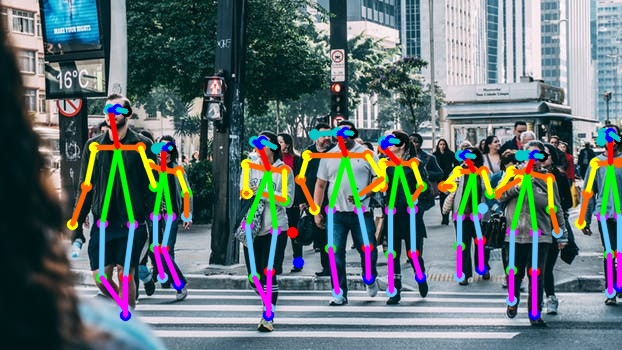
\includegraphics[width=.8\linewidth,height=4cm]{keypoint}  
		\caption{Ejemplo estimación de la postura.}
		\label{fig:keypoint}
	\end{subfigure}
	\begin{subfigure}{.5\textwidth}
		\centering
		% include second image
		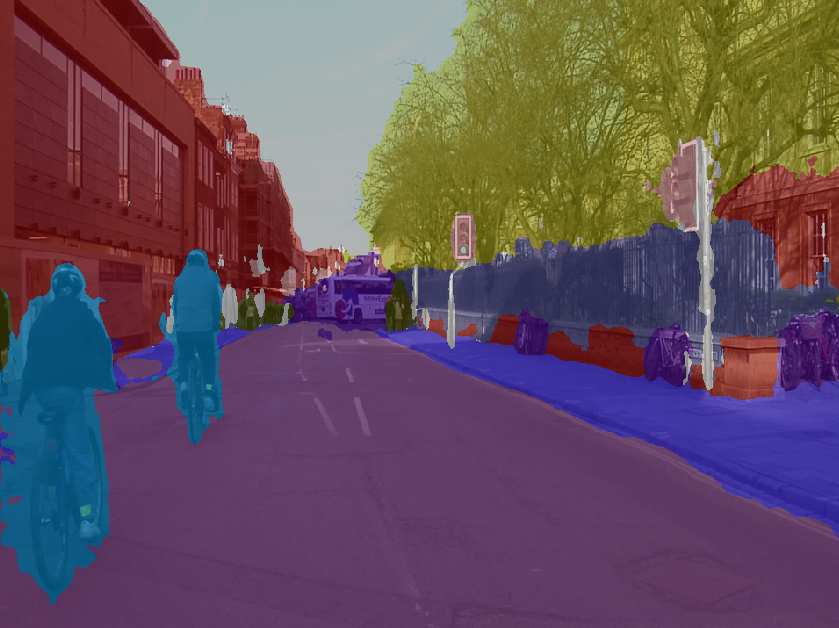
\includegraphics[height=4cm]{segmentacion}  
		\caption{Ejemplo segmentación.}
		\label{fig:segmentation}
	\end{subfigure}
	\caption{Ejemplos tipos de utilidades de la visión por computador.}
	\label{fig:vc}
\end{figure}

\section{Redes neuronales}
Son modelos basados en la analogía con la corteza cerebral de los mamíferos, aunque no están cerca, al menos de momento, de ser tan complejos como el cerebro biológico. El funcionamiento de estos modelos es relativamente sencillo, ya que <<solo>> son un conjunto de unidades básicas (también llamadas neuronas), que reciben una entrada y devuelven una salida. Donde realmente reside su complejidad, al igual que en el cerebro humano, es en las conexiones de estas unidades básicas para formar un modelo complejo capaz de realizar multitud de tareas~\cite{cnn}.

Estas unidades interactúan con los datos que les llegan con una función de activación que puede excitar a esta unidad o neurona y así pasar la información modificada a sus conexiones. Además, las distintas conexiones entre las unidades tienen un peso definido, que expresa la fuerza del enlace. Este peso se modifica a lo largo del entrenamiento de la red para poder obtener mejores resultados.

Según como se propague la información por la red, estas pueden dividirse en dos tipos:
\begin{itemize}
	\item \textbf{\textit{Feed-forward networks}:} redes neuronales donde la información solo avanza por ésta hacia delante, no existe ningún tipo de bucle entre las conexiones de las unidades que haga pasar la información dos o más veces por una de éstas. En este tipo de redes neuronales se encuentran el perceptrón multicapa y las redes neuronales convolucionales
	\item \textbf{\textit{Feed-back networks}:} redes neuronales que sí admiten bucles entre sus conexiones, lo que les permite tener capacidad de memorización. Algún ejemplos de este tipo de redes son las redes neuronales recurrentes o las \textit{Long-Short Term Memory}~\cite{lstm}.
\end{itemize}
\subsection{Redes neuronales convolucionales}
Las redes neuronales convolucionales o CNNs~\cite{cnn}, de sus siglas en inglés Convolutional Neural Network, son de los tipos de redes más usados en la actualidad, sobre todo cuando se trabaja con datos de alta dimensionalidad, principalmente imágenes y vídeos. Las redes neuronales convolucionales tienen dos fases (figura~\ref{fig:cnn}):
\begin{enumerate}
	\item Fase de extracción de características.
	\item Fase de clasificación, puede realizarse con un perceptrón multicapa por ejemplo.
\end{enumerate}

\begin{figure}[h]
	\centering
	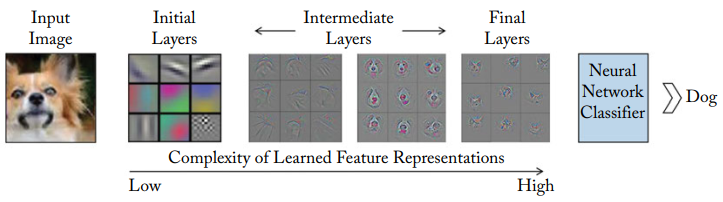
\includegraphics[width=1\textwidth]{cnn}
	\caption{Organización de una red neuronal convolucional~\cite{cnn}.}
	\label{fig:cnn}
\end{figure}

Cada fase está relacionada con un paradigma de aprendizaje distinto, ya que en la extracción de características a partir de filtros se realiza de forma no supervisada, mientras que en la fase de clasificación se realiza un aprendizaje supervisado a partir de los datos obtenidos en la fase de extracción de características.


Aun así, el primer paso que siempre se ha de llevar a cabo antes de entrar en las distintas capas es realizar un preprocesado de la imagen. Éste puede ser por:
\begin{itemize}
	\item Extracción de la media, para a partir de ésta poder centrar los datos. Para cada dato de entrenamiento $x$ de un conjunto $N$ tal que $x \epsilon \mathbb{R}^{h*w*c}$, donde $h$ es el alto de la imagen, $w$ es el ancho y $c$ es color (normalmente 3 dimensiones, RGB), se puede definir la extracción de la media con la siguiente fórmula:
	\begin{equation}
	x'=x-\widehat{x}, \widehat{x}=1/N\sum_{i=1}^{N}x_i
	\end{equation}
	\item Normalización. Con la fórmula:
	\begin{equation}
	x''=\frac{x'}{\sqrt{\frac{\sum_{i=1}^{N}(x_i-\widehat{x})^2}{N-1}}}
	\end{equation}
	\item Blanqueo con PCA para reducir las correlaciones entre las diferentes dimensiones de los datos a partir de un normalización independiente para cada una de ellas.
	\item \textit{Local Contrast Normalization}, tipo de normalización que permite resaltar los valores más elevados.
\end{itemize}

Los tipos de preprocesados que se suelen realizar son las extracción de la media y la normalización, que a la vez son los métodos más sencillos.

\subsubsection{Tipos de capas en una red neuronal convolucional}
\textbf{Capas convolucionales}

Como ya se ha comentado, la funcionalidad de estas capas es la extracción de características a partir de filtros, pero ¿qué es un filtro? Un filtro es una malla con valores discretos, normalmente cuadrada, que representan pesos que se modifican en la fase de entrenamiento de la red. Es con cada uno de estos filtros con los que se recorren los datos para obtener como resultado un resumen de los datos de entrada. Como se ve en la figura~\ref{fig:filtro}, el resumen se calcula aplicando el filtro a los datos multiplicando los valores de los datos por su posición en el filtro y luego sumando los valores.

Al aplicar el filtro hay que tener en cuenta el \textit{stride}, que es el movimiento que hace el filtro en cada paso, en la imagen se puede ver como este valor es de 1 por lo que la imagen avanza horizontal y verticalmente de uno en uno. Valores más altos de \textit{stride} producen resúmenes más comprimidos pero puede que menos precisos, lo que se suele llamar un submuestreo de los datos.

\begin{figure}[h]
	\centering
	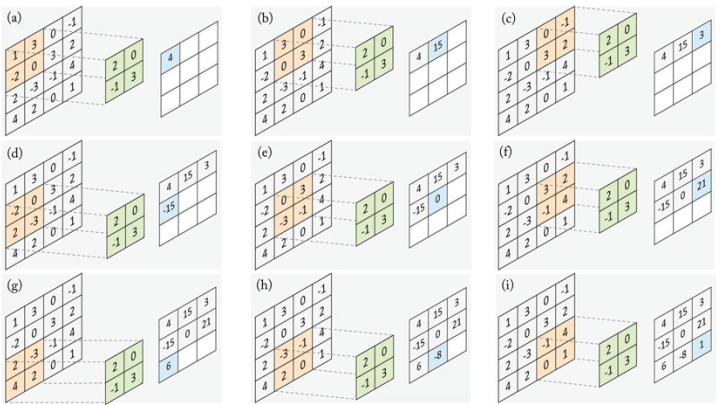
\includegraphics[width=1\textwidth]{filtro}
	\caption{Ejemplo aplicación de un filtro con \textit{stride} 1~\cite{cnn}.}
	\label{fig:filtro}
\end{figure}

Para calcular el tamaño de los datos una vez pasado un filtro se puede usar la siguiente fórmula, donde $h$ es \textit{height} (alto), $w$ es \textit{width} (ancho), $s$ es el \textit{stride} y $f$ es el tamaño del filtro:
\begin{equation}
h'=\left \lfloor \frac{h-f+s}{s} \right \rfloor; w'= \left \lfloor \frac{w-f+s}{s} \right \rfloor
\end{equation}

Siendo $\left \lfloor  \right \rfloor$ la función de parte entera o \textit{floor operation}. Si se aplica esta fórmula a los datos de la imagen~\ref{fig:filtro}:

\begin{equation}
h'=\left \lfloor \frac{4-2+1}{1} \right \rfloor = 3; w'= \left \lfloor \frac{4-2+1}{1} \right \rfloor=3
\end{equation}

Con este tipo de capas existe un problema, ya que hay muchas situaciones que necesitan que se conserve el tamaño de los datos, como por ejemplo en una segmentación, pero si se utiliza este tipo de capas aunque se use el valor mínimo, \textit{stride} 1, se siguen perdiendo datos suavizando sobre todo los bordes. Es por ello que surgió el concepto \textit{zero-padding} que permite mantener el tamaño original de los datos.

El \textit{zero-padding} consiste añadir a los datos de entrada bordes con valores 0 para que cuando se pase el filtro el tamaño de los datos se intente mantener constante. Con el uso del \textit{zero-padding} la fórmula se modifica usando $p$ como el número de aumentos con valores a 0 en cada dimensión~\cite{zeropadding}:
\begin{equation}
h'=\left \lfloor \frac{h-f+s+p}{s} \right \rfloor; w'= \left \lfloor \frac{w-f+s+p}{s} \right \rfloor
\end{equation}

El uso de \textit{padding} se puede dividir en 3 categorías:
\begin{itemize}
	\item \textit{Valid Convolution}: es el caso más sencillo, el filtro siempre se mantiene en posiciones válidas. Las dimensiones finales se reducen tanto en el alto ($h$) como en ancho ($w$) en el tamaño del filtro ($f$) menos 1.
	\item \textit{Same Convolution}: en este caso los datos de entrada y de salida de la capa tienen el mismo tamaño, para conseguirlo se ha de realizar \textit{zero-padding} correctamente, ya que no se puede dar en todos los casos.
	\item \textit{Full Convolution}: en este caso se utiliza el mayor \textit{padding} posible, que se consigue cuando solo un elemento de los datos de entrada está involucrado en todas las operaciones con el filtro.
\end{itemize}

Como se puede ver, el \textit{stride} y sobre todo el tamaño del filtro a aplicar es muy importante en este tipo de capas, es por ello que definir un buen valor para estos puede ser esencial en el desarrollo del modelo. Por esta razón existe la función de \textit{Receptive Field} que permite descubrir el valor para el tamaño de los filtros (todos los filtros de todas las capas del mismo tamaño) más efectivo. La fórmula del \textit{Effective Receptive Field} para la capa $N$ de las $N$ capas convolucionales es:

\begin{equation}
RF_{eff}^n = f + n*(f-1)
\end{equation}

Pero, como se ha visto, los filtros no suelen tener el mismo tamaño ni el mismo \textit{stride}, es por ello que la función de \textit{Receptive Field} para el tamaño de más de un filtro es:

\begin{equation}
RF_{eff}^n = RF_{eff}^{n-1} + ((f_n -1)* \prod_{i=1}^{n-1}s_i)
\end{equation}

Donde $f_n$ es el tamaño del filtro de la capa $n$, $s_i$ es el valor de \textit{stride} para la capa i, y $RF_{eff}^{n-1}$ representa el \textit{effective receptive field} de la capa anterior.

Como ya se ha comentado, uno de los principales problemas de las capas convolucionales son los valores de los bordes, ya que al aparecer menos en las operaciones de los bordes se ven menos representados en las salidas de las capas. Es por ello que se propuso una modificación de las capas convolucionales llamada \textit{Dilated Convolution}, la cual tiene una dilatación ($d$) siendo esta la distancia entre los valores del filtro a tener en cuenta. Como se puede ver en la figura~\ref{fig:dilated}, donde se obtiene un filtro de tamaño 3 y con una dilatación de 2, los valores de los bordes tienen un mayor peso en la salida de la capa.

\begin{figure}[h]
	\centering
	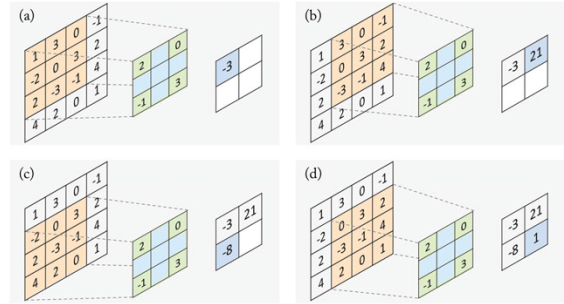
\includegraphics[width=1\textwidth]{dilated}
	\caption{\textit{Dilated Convolution} con dilatación a 2~\cite{cnn}.}
	\label{fig:dilated}
\end{figure}

Al haber añadido un nuevo parámetro, el tamaño de la salida viene dado por las siguiente fórmulas:

\begin{equation}
\begin{split}
h'=\frac{h-f-(d-1)*(f-1)+s+2p}{s}\\w'=\frac{w-f-(d-1)*(f-1)+s+2p}{s}
\end{split}
\end{equation}

\textbf{Capas de agrupación}

Tipo de capa en la cual se realiza una agrupación por un número fijado de datos. Esta agrupación se puede realizar de diversas formas, como puede ser la media, el mínimo o el máximo, entre otros. Como en las capas convolucionales, se ha de pasar el valor del \textit{stride} para indicar cómo va a ser el movimiento del segmento de agrupación. Además, se le ha de pasar el tamaño del segmento de agrupación, algo parecido a lo que pasaba con el tamaño del filtro, pero en este caso no hay valores en el filtro, simplemente se agrupan siguiendo una función los datos del segmento. Un ejemplo se puede ver en la figura~\ref{fig:agrupacion}, donde se puede observar como los valores se van agrupando acorde con el valor máximo del segmento o bloque comprobado. Los tamaños de las salida de los datos tras pasar por una capa se pueden calcular con las siguiente fórmulas, donde $f$ pasa a ser el tamaño del segmento o bloque:

\begin{equation}
h'=\left \lfloor \frac{h-f+s}{s} \right \rfloor;w'=\left \lfloor \frac{w-f+s}{s} \right \rfloor
\end{equation}

\begin{figure}[h]
	\centering
	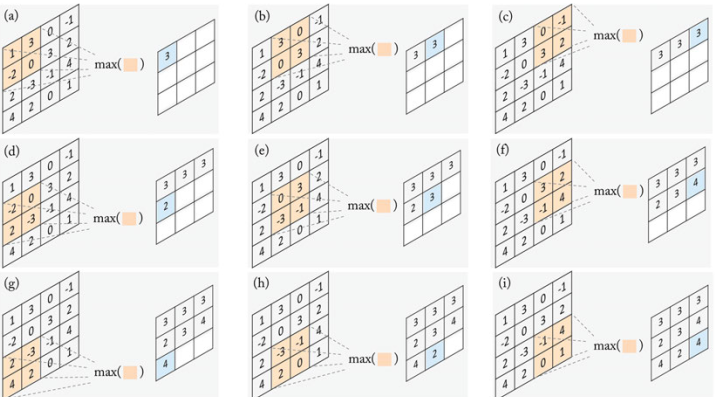
\includegraphics[width=1\textwidth]{agrupacion}
	\caption{Ejemplo de capa de agrupación de tamaño 2~\cite{cnn}.}
	\label{fig:agrupacion}
\end{figure}

Este tipo de capas son muy útiles para compactar la información, para detectar cambios en los datos como puede ser para el movimiento o la posición en una imagen.

\textbf{Capas totalmente conectadas}

Tipo de capa en la cual todas sus unidades están conectadas con todas las unidades de la capa anterior. En este tipo de capas se realiza una operación parecida a las capas convolucionales, salvo que en este caso se realiza con una tamaño de filtro de 1, es decir, se realiza la operación dato a dato. 

\textbf{Capas de no linealidad}

Capas en las cuales la función de activación de cada unidad toma como valor de entrada un número y da como salida un valor en un rango corto, como puede ser [0,1] o [-1,1]. Este tipo de capas suele ir después de las capas <<pesadas>> como las capas convolucionales o de las capas totalmente conectadas. Este tipo de capa es muy importantes utilizarlas después de las capas <<pesadas>> debido a que permite mapear espacios no lineales. Algunas de las funciones de activación de esta capa más comunes se pueden ver en la figura~\ref{fig:funac}.

\begin{figure}[h]
	\centering
	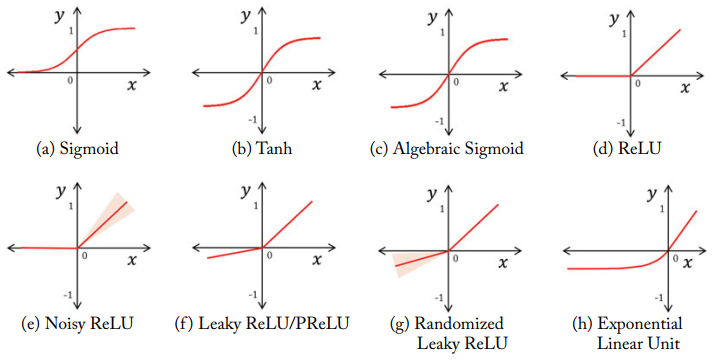
\includegraphics[width=1\textwidth]{funac}
	\caption{Funciones de activación más comunes en capas de no linealidad~\cite{cnn}.}
	\label{fig:funac}
\end{figure}
\subsection{ResNet}
ResNet o \textit{Residual Network} es un tipo de arquitectura de redes neuronales convolucionales creada por Microsoft~\cite{resnet}. Este tipo de CNN se caracterizan por saltarse las conexiones de identidad en los bloques residuales, para así obtener un modelo mucho más sencillo de entrenar. En un bloque residual, los datos de entrada se duplican, pasando unos por las transformaciones y otros por las conexiones de identidad, estas conexiones, como se puede ver en la figura~\ref{fig:resnet}, sirven para saltarse las capas de transformación, pasando los datos iniciales tal cual llegan.

\begin{figure}[h]
	\centering
	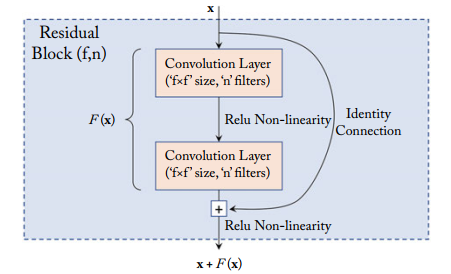
\includegraphics[width=0.5\textwidth]{resnet}
	\caption{Ejemplo bloque residual en ResNet~\cite{cnn}.}
	\label{fig:resnet}
\end{figure}
\subsection{Region-Based CNN}
Las \textit{Region-Based Convolutional Neural Nwtworks} o RCNN son un tipo de redes neuronales convolucionales orientadas al reconocimiento de objetos en imágenes. Este tipo de redes convolucionales, como se puede observar en la figura~\ref{fig:rcnn}, tiene 3 módulos~\cite{cnn}:
\begin{itemize}
	\item Módulo de extracción de propuestas a región.
	\item Módulo de extracción de características. Uso de redes neuronales convolucionales para la extracción de características de cada región propuesta.
	\item Módulo de clasificación de regiones. Se entrena un SVM (Support Vector Machine) por cada clase a predecir, después se usa para clasificar las regiones a partir de las características extraídas en el módulo anterior.
\end{itemize}
\begin{figure}[h]
	\centering
	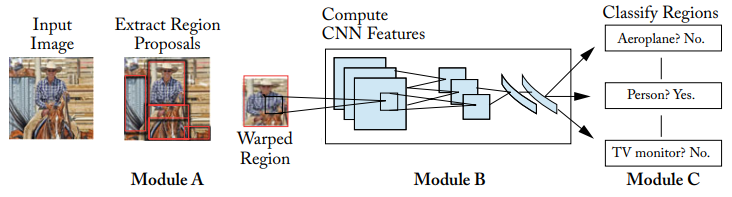
\includegraphics[width=1\textwidth]{rcnn}
	\caption{Region-Based CNN~\cite{cnn}.}
	\label{fig:rcnn}
\end{figure}
\subsection{FPN}
FPN o Feature Pyramid Network es un tipo de red neuronal piramidal que se utiliza junto con las redes neuronales convolucionales para tareas relacionadas con las imágenes, tales como la detección de objetos (usándose junto una RCNN) o la segmentación. Este tipo de redes, como se puede observar en la figura~\ref{fig:fpn}, tiene dos fases~\cite{fpn}:
\begin{itemize}
	\item \textit{Bottom-up pathway}: Fase en la cual se utiliza la red neuronal convolucional para extraer características de la imagen, como por ejemplo con ResNet. Cada capa dentro de esta red neuronal convolucional es de la mitad del tamaño que la anterior (por lo que hay que tener en cuenta todos los atributos de las capas de una red neuronal ya comentados). En el ejemplo de ResNet se obtiene la salida de cada capa como el resultado de cada bloque residual.
	\item \textit{Top-down pathway and lateral connections}: En esta fase, en el primer nivel, se toma como entrada la salida de la última capa de la fase anterior, y se va bajando de nivel pasando al siguiente nivel la predicción del anterior y la salida de la capa de la red neuronal que está al mismo nivel.
\end{itemize}
\begin{figure}[h]
	\centering
	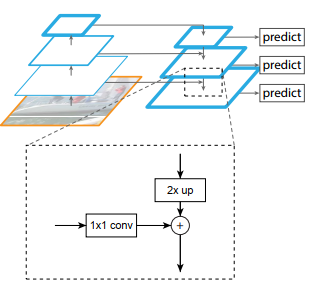
\includegraphics[width=0.5\textwidth]{fpn}
	\caption{Feature Pyramid Network~\cite{fpn}.}
	\label{fig:fpn}
\end{figure}

\section{Puntos y vectores}
El punto es la representación mínima en una espacio, donde representa una posición exacta dentro de este espacio. Un punto dentro de un espacio se representa con tantos valores como dimensiones tiene el espacio donde se encuentra.

El vector es otro de los conceptos básicos matemáticos que se define como un segmento orientado. Un vector se representa a partir de 3 valores, su módulo o longitud del segmento, su dirección y su sentido.

Este concepto de vector, o incluso conceptos con mayor número de dimensiones como son las matrices, es muy utilizado en la programación. Uno de los tipos más conocidos de matrices multidimensionales que trabaja con solo un tipo de dato son los \textit{tensors}, matrices multidimensionales implementadas para optimizar las operaciones en la GPU (tarjeta gráfica)~\cite{tensor}. 

\subsection{Distancia entre puntos}
La distancia entre dos puntos es el espacio que los separa. Esta distancia se puede calcular de distintas formas, ya que depende mucho del espacio en el que se encuentren los puntos. Algunas de las distancias más comunes son:
\begin{itemize}
	\item \textbf{Manhattan}: distancia que se calcula como la suma de las diferencia de los valores de las distintas dimensiones de los puntos.
	\item \textbf{Euclídea}: distancia que se calcula como la longitud de la línea que une los dos puntos, a partir del teorema de Pitágoras.
\end{itemize}

\subsection{Ángulo entre vectores}
Ángulo mínimo que hay que girar un vector para conseguir la dirección del otro vector con el cual ha de compartir al menos un punto~\cite{angvec}.

\capitulo{4}{Técnicas y herramientas}

Esta parte de la memoria tiene como objetivo presentar las técnicas metodológicas y las herramientas de desarrollo que se han utilizado para llevar a cabo el proyecto. Si se han estudiado diferentes alternativas de metodologías, herramientas, bibliotecas se puede hacer un resumen de los aspectos más destacados de cada alternativa, incluyendo comparativas entre las distintas opciones y una justificación de las elecciones realizadas. 
No se pretende que este apartado se convierta en un capítulo de un libro dedicado a cada una de las alternativas, sino comentar los aspectos más destacados de cada opción, con un repaso somero a los fundamentos esenciales y referencias bibliográficas para que el lector pueda ampliar su conocimiento sobre el tema.



\capitulo{5}{Aspectos relevantes del desarrollo del proyecto}

Este apartado pretende recoger los aspectos más interesantes del desarrollo del proyecto, comentados por los autores del mismo.
Debe incluir desde la exposición del ciclo de vida utilizado, hasta los detalles de mayor relevancia de las fases de análisis, diseño e implementación.
Se busca que no sea una mera operación de copiar y pegar diagramas y extractos del código fuente, sino que realmente se justifiquen los caminos de solución que se han tomado, especialmente aquellos que no sean triviales.
Puede ser el lugar más adecuado para documentar los aspectos más interesantes del diseño y de la implementación, con un mayor hincapié en aspectos tales como el tipo de arquitectura elegido, los índices de las tablas de la base de datos, normalización y desnormalización, distribución en ficheros3, reglas de negocio dentro de las bases de datos (EDVHV GH GDWRV DFWLYDV), aspectos de desarrollo relacionados con el WWW...
Este apartado, debe convertirse en el resumen de la experiencia práctica del proyecto, y por sí mismo justifica que la memoria se convierta en un documento útil, fuente de referencia para los autores, los tutores y futuros alumnos.

\capitulo{6}{Trabajos relacionados}

La rehabilitación de pacientes con problemas físicos o mentales ha evolucionado en los últimos años, gracias a los avances tecnológicos, a un sistema de rehabilitación \textit{online}, que como se explicó en la introducción del trabajo, permite habilitar estos sistemas de rehabilitación a pacientes que por diversas razones no pueden desplazarse a las consultas médicas a realizar esta rehabilitación para mejorar sus situación.

La aparición de las rehabilitaciones \textit{online} está permitiendo la automatización de estos sistemas. Gracias a herramientas de visión por computador permiten, sin la presencia de un médico especializado, dar una retroalimentación al paciente de los ejercicios que realiza.

A continuación, se van a comentar algunos de los proyectos, que como el proyecto que se ha desarrollado en este Trabajo Fin de Máster, han desarrollado un sistema que utiliza la visión por computador para mejorar las rehabilitaciones de pacientes.

\subsection{A Kinect-based system for cognitive rehabilitation exercises monitoring~\cite{kinectbasedsystem}}
En este artículo de la Universidad de Valladolid se puede observar el uso de técnicas de visión por computador para calcular características como el tiempo de reacción de los pacientes con algún problema físico o personas que confunden el lado derecho e izquierdo de su cuerpo, y seguir los movimientos del paciente.

Los ejercicios en los que se centra este proyecto se centran en movimientos de la mano hacia la cabeza, para ello utilizan la estimación de posición, en 3D, que les ofrece la cámara \textit{Kinect}. Kinect es una cámara desarrollada por \textit{Microsoft} que originalmente se diseñó desde un enfoque lúdico para la vídeo consola \textit{Xbox 360}, pero que ha terminado siendo una de las mejores cámaras para su uso en visión por computador~\cite{wiki:kinect}. Actualmente, con la nueva generación de la vídeo consola de \textit{Microsoft} (\textit{Xbox One}) salió en 2013 una nueva versión de su cámara \textit{Kinect}.

Para poder monitorizar estos ejercicios, se realiza una estimación y seguimiento de los rasgos faciales (ojos, nariz y orejas) y de las manos derecha e izquierda. Para realizar este proceso se utiliza la estimación de la posición dada por \textit{Kinect} y el uso de modelos predictivos como \textit{AdaBoost}~\cite{ada} para la detección de la cara, de la cual posteriormente se los rasgos faciales (el esqueleto proporcionado por \textit{Kinect} solo aporta la posición de la cabeza, no de los rasgos faciales).

En este proyecto se trabajó con vídeos de 640 × 480 píxeles con 13 fotogramas por segundo, con un tiempo medio de estimación de las posiciones necesarias de 79 milisegundos, realizado en Visual C++ en un dispositivo con un procesador de 3 GHz. La evaluación de los ejercicios se realiza de manera \textit{offline} una vez termina el ejercicio. 

Cabe destacar que este proyecto se desarrolló con la finalidad de ser incluido en \textit{GRADIOR}\footnote{\textit{GRADIOR}: \url{https://ides.es/gradior}}, plataforma virtual para la estimulación cognitiva, evaluación y rehabilitación neuropsicológica~\cite{gradior}.

\subsection{Computer Vision-Based Classification of Hand Grip Variations in Neurorehabilitation~\cite{hand}}
En este proyecto se realizó un sistema de visión por computador, que puede usarse con realidad virtual, para la clasificación de posturas de las manos en la rehabilitación de pacientes.

Para poder obtener mayor información para detectar correctamente la postura de la mano se utilizan dos cámaras, una que graba el lateral de la mano, y otra que graba la parte superior de ésta (figura~\ref{fig:hand}). Las cámaras capturan con una frecuencia de 15 fotogramas por segundo a una resolución de 352 $\times$ 288 píxeles.

\begin{figure}[ht]
	\centering
	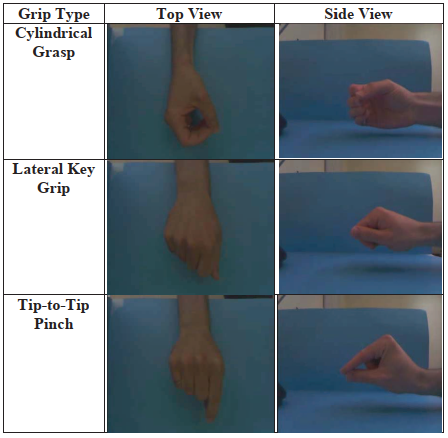
\includegraphics[width=0.65\textwidth]{handeee}
	\caption[Ejemplos cámaras en rehabilitación de manos.]{Ejemplos cámaras en rehabilitación de manos~\cite{hand}.}
	\label{fig:hand}
\end{figure}

Para el procesado de las imágenes se usa una librería de C++ llamada OpenCV. Con esta librería se quita el fondo de la imagen para dejar solo a la mano (con técnicas de comparación de colores, erosión y dilatación de la imagen). Sobre esta imagen procesada se obtiene:
\begin{itemize}
	\item Los siete \textit{Hu invariant moments} sobre una versión de escala de grises de la imagen~\cite{humingkuei2011}.
	\item Contorno de la mano.
	\item Contorno interior en los casos necesarios, cuando la mano hace la forma de un agujero.
\end{itemize}

La clasificación final de las posturas se realiza con estos datos utilizando \textit{k-Nearest Neighbors} (\textit{kNN}), calculado con los 20 vecinos más cercanos ($k=20$).

\subsection{A Computer Vision System for Virtual Rehabilitation~\cite{bonen}}
En este proyecto se utiliza la segunda versión de la cámara de \textit{Microsoft}, \textit{Kinect}, para la mejora en la estimación de la postura y el seguimiento del movimiento en personas con deficiencias motoras. Esta mejora se consigue utilizando las distintas cámaras de \textit{Kinect V2} y juntando toda esa información para obtener el mejor esqueleto posible en 3D. Además, el proyecto ha sido desarrollado para ser usado con realidad virtual con \textit{Oculus RIFT 2 HMD}.

Este proyecto destaca por el uso de 4 \textit{Kinect V2} puestas en las esquinas de la habitación conectadas a un \textit{Intel Next Unit of Computing} (\textit{NUC}) que permite preprocesar las imágenes, solo unos pocos puntos son mandados al ordenador maestro (\textit{Master PC}) para crear el esqueleto (figura~\ref{fig:4kinects}).

\begin{figure}[h]
	\centering
	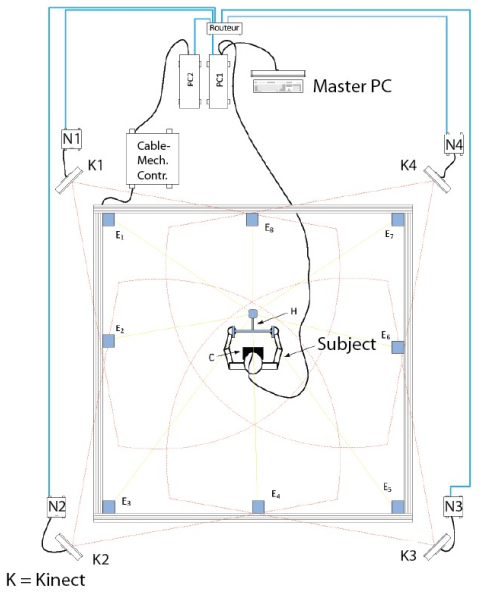
\includegraphics[width=0.5\textwidth]{4kinect}
	\caption[Disposición \textit{Kinects V2}(\textit{K}), \textit{NUC}(\textit{N}) y el \textit{Master PC}.]{Disposición \textit{Kinects V2}(\textit{K}), \textit{NUC}(\textit{N}) y el \textit{Master PC}~\cite{bonen}.}
	\label{fig:4kinects}
\end{figure}

En el \textit{paper} los creadores comentan que la estimación de la posición de \textit{Microsoft} es muy buena, pero que al tener 4 \textit{Kinects V2} se tiene que juntar y aplicar unos filtros para el correcto funcionamiento.

Además, en el \textit{paper} se describen dos formas de ejecutar la estimación de la posición desarrollada, una versión en <<tiempo real>> que permite mandar la información del esqueleto directamente a las \textit{Oculus}, y una versión \textit{offline} de mayor precisión pero con la necesidad de un postprocesado de la información obtenida.


\subsection{Conclusiones}
Todos estos proyectos, cada uno orientado y elaborado de una forma distinta, muestran lo valioso que puede llegar a ser la introducción de la tecnología en la rehabilitación de pacientes con problemas físicos e incluso mentales. Este valor añadido ofrece, además de una reducción en costes y en intervención humana, una mejoría en la vida de los pacientes ya que realizan más rehabilitaciones que hacen sus vidas más llevaderas~\cite{motiv}.

\capitulo{7}{Conclusiones y Líneas de trabajo futuras}

En este apartado se encuentran las conclusiones finales del proyecto, así como el conjunto de tareas y/o mejoras que se podrían realizar.

\section{Conclusiones}
El proyecto se ha desarrollado en una situación anómala. Con la irrupción de la \textit{COVID-19} y el correspondiente confinamiento se limitó mucho el desarrollo orientado al paciente que se estaba dando en las primeras fases del desarrollo de la aplicación de rehabilitación \textit{online}. Con suerte, para mediados de febrero ya existía una primera versión de esta aplicación.

La imposibilidad de realizar instalaciones de dispositivos impidió la recolección de datos (vídeos) con los que poder implementar un modelo propio de visión artificial. Aunque al realizar el estudio del estado del arte sobre las herramientas existentes se vio que hubiese sido muy complicado la creación de uno de estos modelos, principalmente por limitaciones en el \textit{hardware}. Aun así, el estudio del estado del arte realizado ha dado muy buenos resultados, encontrando una herramienta muy buena que permite realizar las tareas de visión por computador en unos tiempos admisibles.

A partir del estudio de las herramientas y con la obtención del modelo final se pudo estudiar e implementar un sistema de extracción de características de la salida del modelo, con el que posteriormente se desarrolló la comparación de posiciones. Aun con la dificultad de no poder realizar reuniones presenciales para comentar el proceso del desarrollo con el equipo médico, sí que se realizaron reuniones de manera \textit{online} y se recibieron vídeos de ejercicios de ejemplos que fueron tomados como muestra para realizar la comparación de posiciones. 

Con todas estas tareas realizadas se cumplió con todos los objetivos marcados al principio del proyecto, incluso superando con creces algunas expectativas sobre el funcionamiento del estimador de posiciones y de los tiempos de ejecución en un problema tan complejo y con una gran cantidad de datos muy pesados.

Actualmente, con la vuelta a la normalidad se está volviendo a realizar instalaciones de dispositivos con los cuales se están recogiendo los primeros datos. Gracias al proyecto, los pacientes con \textit{Parkinson} no necesitarán desplazarse para realizar sus rehabilitaciones y podrán realizarlas de una manera más frecuente con el sistema de retroalimentación de sus ejercicios y evoluciones. Además, con la implementación extensible realizada con la configuración de las comparaciones, estas implementaciones se pueden utilizar para distintos tipos de ejercicios y de enfermedades. 

Por último, cabe destacar el interés por parte de la OTRI--Transferencia (servicio de la Universidad de Burgos centrado en el desarrollo de ideas y del fomento del emprendimiento en los estudiantes) al recibir el premio prototipo de la edición 2019-2020\footnote{Resolución Premios Prototipo 2019-2020: \href{https://www.ubu.es/te-interesa/convocatoria-prototipos-orientados-al-mercado-curso-2019-2020}{https://www.ubu.es/te-interesa/convocatoria-prototipos-orientados-al-mercado-curso-2019-2020}.}. Gracias a este premio se pudo asistir a distintos talleres de comunicación y presentación de proyectos, marketing digital y de propiedad industrial. Además, se recibió un asesoramiento sobre estos ámbitos.

\section{Líneas de trabajo futuras}
Como se ha comentado, la principal línea de trabajo futura, que ya se está trabajando pero que no entra en este Trabajo Fin de Máster, es la incorporación del proyecto del compañero José Luis Garrido Labrador y este proyecto a la aplicación \textit{web}. Para así permitir a los pacientes realizar ejercicios de forma autónoma.

Aun así, las principales líneas futuras de trabajo orientadas al desarrollo único de este proyecto son:
\begin{itemize}
	\item Poder probar a crear un modelo propio de visión artificial. Por insuficiencia de datos esta meta no se pudo siquiera plantear.
	\item Contar con un mayor presupuesto que permita obtener cámaras de mayor calidad como pueden ser las \textit{Kinect V2} que permiten la obtención de la posición en 3D y mejores ordenadores en las casas de los pacientes que permitan realizar un preprocesado o incluso la extracción de la posición. Convirtiendo así el flujo de vídeos en un flujo de posiciones con un tamaño considerablemente menor, lo que permitiría mejorar los tiempos del flujo aun más.
	\item Extraer mayor información más allá de la comparación de ejercicios, como puede ser el tiempo de reacción de los pacientes.
	\item Implementar en paralelo un predictor de caídas. Los pacientes de \textit{Parkinson} suelen sufrir de caídas debido a las limitaciones en su sistema motor. Por ello un sistema capaz de predecir la caída del paciente para poder detener el ejercicio o incluso alertar a algún familiar o conocido.
\end{itemize}




%\renewcommand\chaptername{Anexo}
%\renewcommand\thechapter{\Roman{chapter}}
%\setcounter{chapter}{0}

% Añadir entrada en el índice: Anexos
\appendix
\addcontentsline{toc}{part}{Apéndices}
\part*{Apéndices}

\apendice{Plan de Proyecto Software}

\section{Introducción}
La planificación de un proyecto es una fase esencial en desarrollo de éste, ya que permite comprobar y guiar el proyecto según las necesidades actuales y futuras.

Dentro de este plan para el desarrollo del proyecto se pueden diferenciar dos puntos sobre los que se puede enfocar este estudio:
\begin{itemize}
	\item \textbf{Temporal}: enfoque en el que se analiza la evolución del proyecto en el tiempo. Al utilizar una metodología SCRUM, se ha divido el desarrollo en \textit{sprints} de 2 semanas.
	\item \textbf{Viabilidad}: comprobación de la adecuación del proyecto tanto desde el ámbito económico como desde el ámbito legal.
\end{itemize}
\section{Planificación temporal}
Como ya se ha comentado, la planificación temporal se ha divido en distintos \textit{sprints} de 2 semanas cada uno, en lo cuales se realizaron distintas tareas y reuniones. Cabe destacar que antes de realizar el primer \textit{sprint} se desarrolló la aplicación FIS sobre la cuál será implementado en el futuro el proyecto desarrollado.

\subsection{\textit{Sprint}0}
En este \textit{sprint} se creó la aplicación para el Hospital Universitario de Burgos llamada FIS-HUBU. Esta aplicación, como se ha visto en el apartado~\ref{desarrolloFH}, sirve para realizar vídeo llamadas entre médicos y los pacientes con Parkinson en las cuales se realizan rehabilitaciones para mejorar su calidad de vida. Como se ha explicado, esta aplicación cuenta con dos partes, una para los médicos o responsables y otra para los pacientes. Las tareas realizadas en este \textit{sprint} son las siguientes:
\begin{itemize}
	\item Investigación sobre plataformas de vídeo llamadas.
	\item Creación de la estructura base de la página web.
	\item Diseño e implementación de la base de datos.
	\item Creación del login por usuario, guardando una \textit{cookie} para mantener la sesión.
	\item \textit{Backend} de las páginas de los pacientes, donde se  incluye la creación de las llamadas, el calculo de la evolución a partir de los datos en la base de datos, la grabación de la cámara del paciente y subida a un servidor propio de la universidad...
	\item \textit{Backend} de las páginas de los responsables.
\end{itemize}

Tras desarrollar la aplicación se empezaron con las tareas de explotación de la aplicación, en donde se cogieron los dispositivos para los paciente y se les instalaron todo el \textit{software} necesario para funcionar correctamente, y con ello poder grabar los vídeos y subirlos a un servidor propio. Debido a la aparición del COVID-19 y el posterior confinamiento sufrido y las consiguientes medidas de seguridad no se pudo empezar a instalar los dispositivos en las casa de los pacientes.
\subsection{\textit{Sprint} 1: 17/02/2020 - 26/02/2020}
Este es el primer \textit{sprint} real del desarrollo de la parte del proyecto de visión artificial, en el se realizaron las primeras tareas de creación del repositorio en \textit{GitHub} y la creación de la estructura del mismo. Además, se creo el documento \LaTeX{} a partir de la plantilla de la asignatura. Las tareas más relevantes en este primer \textit{sprint} fueron las relacionadas con la configuración de \textit{Gamma} y los primeros pasos en la investigación de algoritmos de visión por computador y detección de movimiento, como son \textit{Detectron2} y \textit{PoseNet}.
\subsection{\textit{Sprint} 2: 27/02/2020 - 11/03/2020}
En este \textit{sprint} se realizó una tarea fundamental dentro del desarrollo del proyecto, que es la investigación y elección del algoritmo de visión artificial para la obtención de la postura, que se usará en los fotogramas de los vídeos recogidos con la aplicación FIS-HUBU y compararlos con otros vídeos base para saber la exactitud del ejercicio. Esta tarea de investigación de los distintos algoritmos dio como resultado que el \textit{Dectectron2} (apartado~\ref{dectectron}) es el algoritmo que más se amoldaba al problema del proyecto.

Además, en este \textit{sprint} se realizaron las tareas de documentación necesarias sobre los algoritmos candidatos y sobre la selección del mejor.
\subsection{\textit{Sprint} 3: 12/03/2020 - 02/05/2020}
En este tercer \textit{sprint} se profundizó en la investigación de los distintos algoritmos y modelos de \textit{Detectron2}. En este \textit{sprint} se realizaron las siguientes tareas:
\begin{itemize}
	\item Documentación de los primeros objetivos del proyecto.
	\item Estudio de la herramienta \textit{Detectron2}.
	\item Estudio de los modelos ya creados en \textit{Detectron2}.
	\item Estudio sobre los modelos de detección de posición de \textit{Detectron2}.
	\item Estudio del \textit{threshold}.
	\item Interpretación de la salida obtenida.
	\item Creación de la clase de posición y extracción de características a partir de los datos devueltos por el modelo.
	\item Documentación de los aspectos relevantes.
\end{itemize}

\section{Estudio de viabilidad}

\subsection{Viabilidad económica}

\subsection{Viabilidad legal}



%\apendice{Especificación de Requisitos}

\section{Introducción}

\section{Objetivos generales}

\section{Catalogo de requisitos}

\section{Especificación de requisitos}



\apendice{Especificación de diseño}

\section{Introducción}
En cualquier proyecto la fase de diseño de las distintas partes de éste es esencial para su correcta implementación, desarrollo y evolución. En este apartado se va a comentar los distintos diseños que se han realizado para poder obtener una solución óptima, aun así hay que tener en cuenta el gran peso que tiene la investigación en este proyecto por lo que el diseño en una gran parte del proyecto no ha sido necesario.

Los diseños realizados en el proyecto han sido:
\begin{itemize}
	\item \textbf{Diseño de datos}: subapartado donde se van a mostrar las distintas estructuras de datos utilizadas, así como un conjunto de diagramas para comprender la estructura de los ficheros de ejecución del proyecto.
	\item \textbf{Diseño procedimental}: subapartado donde se va a mostrar, principalmente, como es la comunicación entre el flujo y las implementaciones realizadas.
\end{itemize}
\section{Diseño de datos}

Este proyecto, al ser mayoritariamente un proyecto de investigación apenas tiene diseño de datos. Aun así, sí que existe un diseño donde se muestra la estructura de los ficheros necesarios para la ejecución final sobre el flujo.

Este diseño se muestra en forma de diagrama de clases, figura~\ref{fig:diacla}, donde los asteriscos en los nombres de las variables representan que realmente hay dos variables una para la parte izquierda y otra para la derecha (un ejemplo puede se el hombro*, que significa que existe un hombroI y un hombroD, los dos del mismo tipo). En el diagrama se muestra la implementación final de la posición con la clase \texttt{Posicion}, que como se comentó en el apartado~\ref{reducida}, es la versión reducida con el conjunto mínimo de cálculos necesarios.

Por otro lado, la clase \texttt{Interfaz} es la que se comunica con el flujo de datos (de ahí su nombre), en ella se carga el modelo y se crean y se comparan las posiciones.

Además, en el diagrama se pueden observar las relaciones entre las clases más usadas en el código. En este diagrama se puede observar también como se incorpora la herramienta \textit{Detectron2} en el proyecto (clases \texttt{cfg}, \texttt{model\_zoo}, \texttt{Instances} y \texttt{DefaultPredictor}).

\begin{landscape}
	\begin{figure}[h]
		\centering
		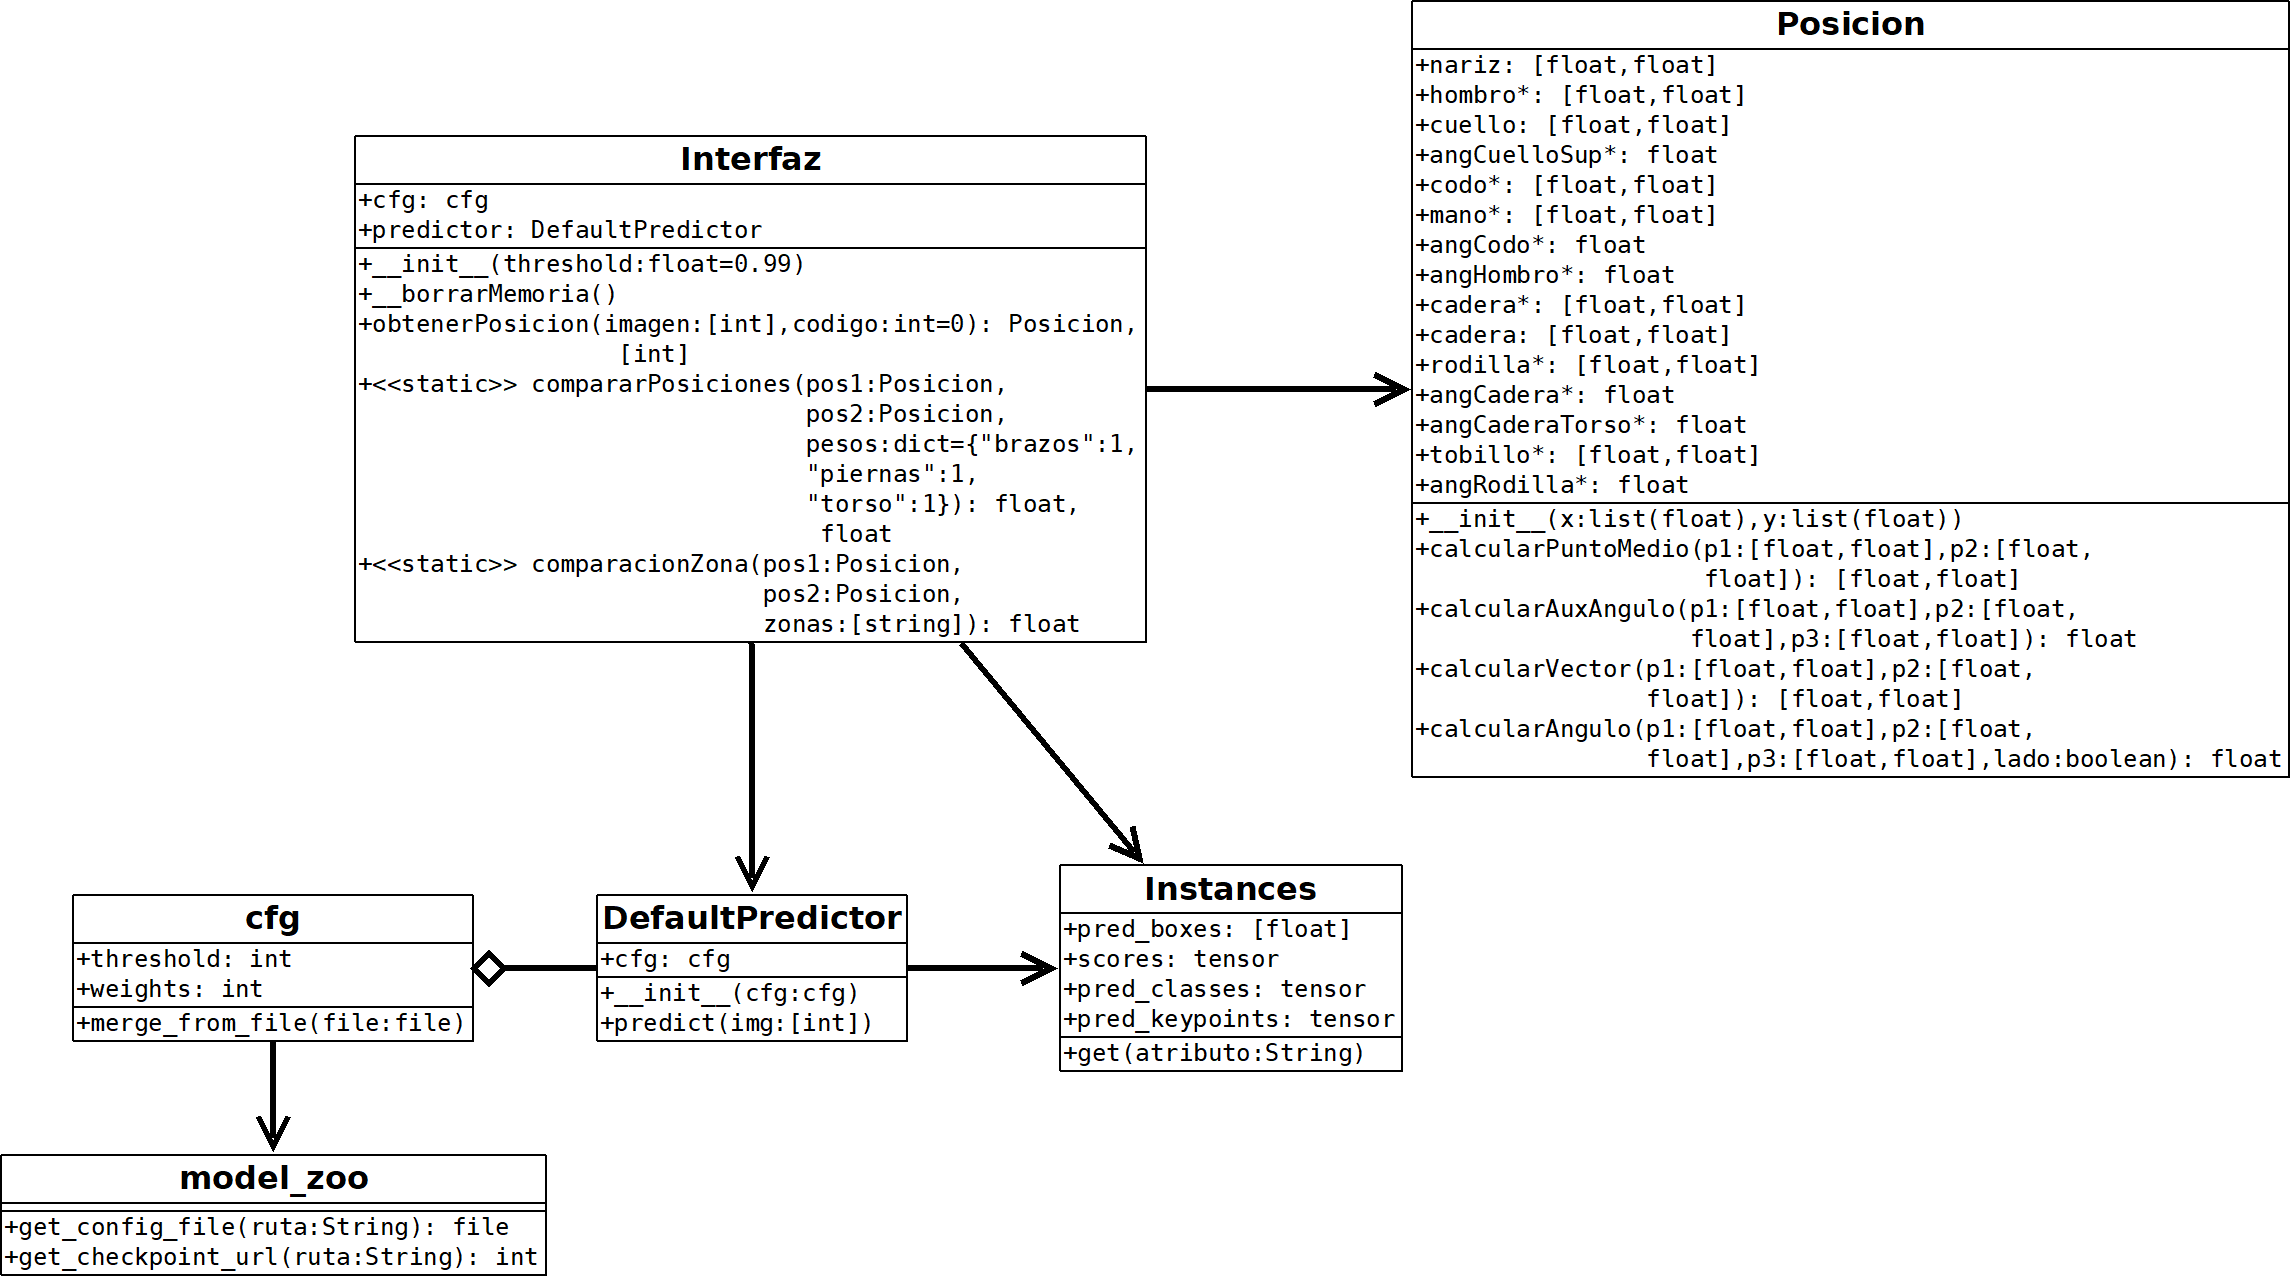
\includegraphics[width=1.6\textwidth]{DiagramaClaseFinal}
		\caption{Diagrama de clases.}
		\label{fig:diacla}
	\end{figure}	
\end{landscape}

\section{Diseño procedimental}

El diseño procedimental realizado en este proyecto, como en el caso del diseño de datos, se ha realizado sobre la implementación final en las clases que usan el flujos de datos. Estos diseño procedimentales se han realizado a partir de diagramas de secuencia, donde se muestran las dos posibbles interacciones del flujo con las clases.

En la primera posibilidad, el flujo tan solo pide las posiciones de las imágenes que va proporcionando, figura~\ref{fig:diasec1}. Como se puede ver en el diagrama de secuencias, lo primero que tiene que realizar un \textit{worker} del flujo es instanciar la clase \texttt{Interfaz} donde se procede con la carga y configuración del modelo. Una vez instanciada la clase, se pueden hacer llamadas para obtener la estimación de la posición de un imagen (operación que se puede repetir mientras esté cargado el modelo, es decir, mientras esté vivo el \textit{worker}).

\begin{figure}[h]
	\centering
	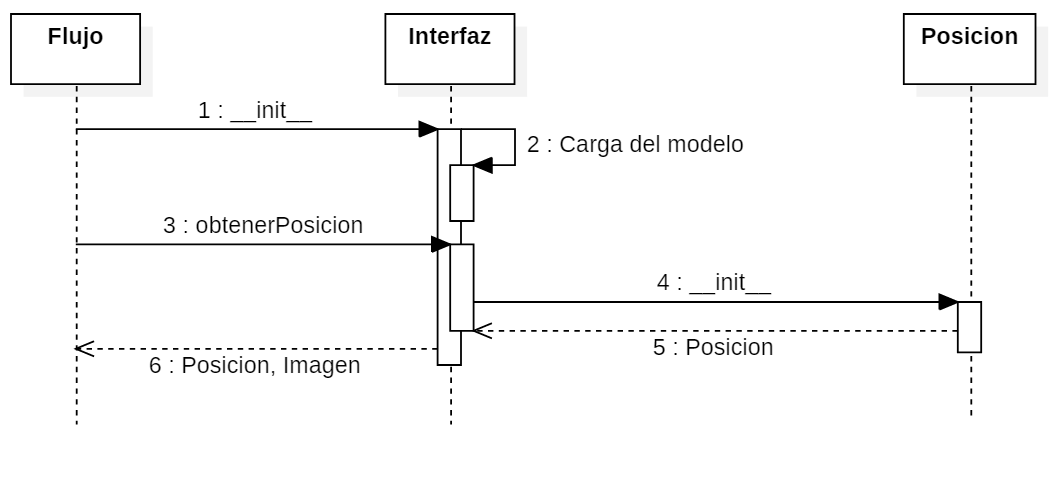
\includegraphics[width=1\textwidth]{DiagramaSecuenciaPosicion}
	\caption{Diagrama de secuencia, estimación posición.}
	\label{fig:diasec1}
\end{figure}

Por otro lado, una segunda posibilidad de la ejecución con el flujo es la comparación de posiciones, figura~\ref{fig:diasec2}. En este diagrama de secuencias se muestra como es la interacción entre los distintos elementos que trabajan con el flujo, como en el caso anterior las llamadas a la comparación y obtención de posiciones se pueden realizar mientras esté vivo el \textit{worker} que tiene el modelo cargado.

\begin{figure}[h]
	\centering
	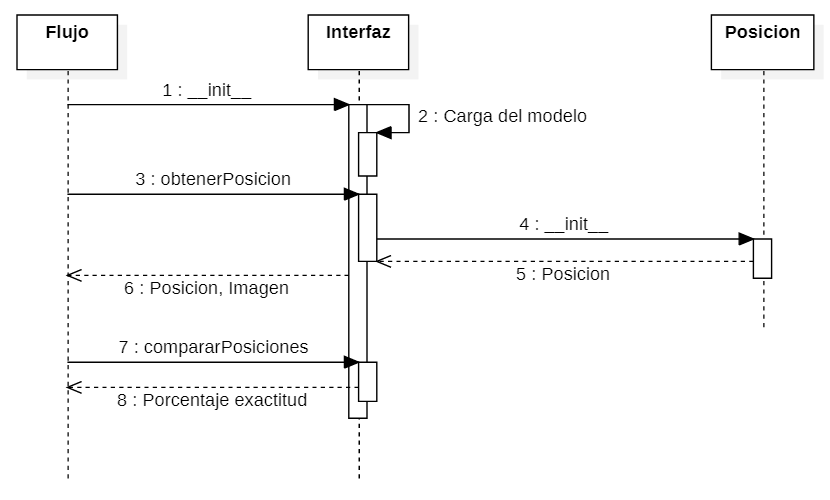
\includegraphics[width=1\textwidth]{DiagramaSecuenciaComparacion}
	\caption{Diagrama de secuencia, comparación de posiciones.}
	\label{fig:diasec2}
\end{figure}



\apendice{Documentación técnica de programación}

\section{Introducción}
En este apartado se detallan los puntos que ha de conocer una persona, con conocimientos en informática, que quiera utilizar los distintos elementos del proyecto. Es por ello que este apartado se divide en los siguientes subapartados:
\begin{itemize}
	\item \textbf{Estructura de directorios}: subapartado donde se comenta la estructura del proyecto. El proyecto además se puede observar en el repositorio de \textit{GitHub}, donde a parte de la estructura y los documentos del proyecto se pueden observar las tareas que se han realizado.
	\item \textbf{Manual del programador}: manual en donde se muestran los pasos a seguir para poder continuar desarrollando el proyecto.
	\item \textbf{Compilación, instalación y ejecución del proyecto}: explicación paso a paso para conseguir utilizar los distintos elementos implementados en el proyectos.
	\item \textbf{Pruebas del sistema}: explicación de las distintas pruebas realizadas en la fase de investigación y de despliegue del proyecto, así como explicación de cómo lanzar estas pruebas.
\end{itemize}
\section{Estructura de directorios}
En este subapartado se va a comentar la estructura y el contenido de los directorios del proyecto que se encuentra subido a un repositorio público en \textit{GitHub}\footnote{Repositorio: \href{https://github.com/Josemi/TFM-FIS-IA}{https://github.com/Josemi/TFM-FIS-IA}}. Empezando con la raíz del proyecto que tiene la siguiente estructura:
\dirtree{%
	.1 /.
	.2 \textbf{src}.
	.2 \textbf{doc}.
	.2 README.md.
	.2 LICENSE.
	.2 .gitignore.
}

Como se puede ver, de la raíz cuelgan dos carpetas, src y doc, y tres documentos que se usan para el repositorio en \textit{GitHub}. La funcionalidad de estos ficheros es:
\begin{itemize}
	\item README.md: documento que permite mostrar información cuando se abre el repositorio en la página de \textit{GitHub}. Este tipo de documentos se encuentran en la mayoría de los directorios del proyecto para informar que se encuentra en ellos.
	\item LICENSE: documento que permite mostrar la licencia del proyecto en \textit{GitHub}.
	\item .gitignore: documento oculto que permite señalar que directorios o ficheros no se quieren subir al repositorio público.
\end{itemize}

\subsection{Documentación}
En cuanto a las carpetas se va a empezar comentando la estructura del directorio \texttt{doc}, directorio donde se encuentra toda la documentación del proyecto, que tiene la siguiente composición:
\dirtree{%
	.1 /doc/.
	.2 \textbf{Diagramas}.
	.2 \textbf{Latex}.
	.2 \textbf{Vídeos}.
}

En el directorio \texttt{Diagramas} se encuentran todos los documentos de diseño realizados para el proyecto, la exportación de estos documentos se encuentra dentro del otro directorio llamado \texttt{Latex}. Para realizar los diseños se han utilizado distintos programas como son DIA~\cite{dia} y StarUML~\cite{staruml}.

En la carpeta \texttt{Vídeos} se encuentran una serie de vídeos que hacen un resumen de la estructura del proyecto, así como muestran alguna ejecución de alguna parte del proyecto.

Por otro lado, la carpeta \texttt{Latex} contiene todos los documentos necesarios para la documentación en \LaTeX{} de la memoria y de los apéndices del proyecto. Cabe destacar que en la carpeta \texttt{/doc/Latex/img} se encuentran las exportaciones de los diagramas comentados, además del resto de imágenes usadas en el documento.

\subsection{Código}
El código de las implementaciones y las pruebas se encuentra en la carpeta \texttt{/src}, de la cual cuelga los siguientes subdirectorios:
\dirtree{%
	.1 /src/.
	.2 \textbf{pruebas}.
	.2 \textbf{pos}.
	.2 \textbf{python-flujo}.
	.2 visualizarComparacion.ipynb.
}

Como se puede observar, hay tres carpetas de código y un fichero \textit{Jupyer Notebook}, las cuales corresponden con:
\begin{itemize}
	\item \textbf{pruebas}: conjunto de pruebas de usadas en \textit{Detectron2} desde la selección del modelo y del \textit{threshold} hasta las pruebas con los problemas con los brazos.
	\item \textbf{pos}: conjunto de ficheros de \textit{Jupyter Notebooks} donde se encuentran las versiones de las posiciones y de la comparación, junto con las pruebas de tiempo de ejecución.
	\item \textbf{python-flujos}: conjunto de ficheros \textit{Python} donde se encuentran todas las versiones implementadas tanto de la posición como de comparación de posiciones. Además, se encuentra el fichero \textit{fishubuia.py} donde se encuentra la implementación que junto con el fichero \textit{PosicionVF.py} permite la ejecución del cálculo de la posición y comparación en el flujo.
	\item \textbf{visualizarComparacion.ipynb}: fichero \textit{Jupyter Notebook} creado para mostrar el funcionamiento de la comparación y aplicar los conocimientos de visualización de datos obtenidos durante diversas asignaturas del máster para mostrar información relevante sobre esta. Con esto también se quiere mostrar la capacidad que tiene el sistema implementado.
\end{itemize}

\section{Manual del programador}
Como se ha explicado, el código final se encuentra en la carpeta \texttt{/src/python-flujo}, donde están todas las versiones de la clase de la posición y todas las versiones de las comparaciones de estas. Además, se encuentra el fichero final que permite, a partir de una clase llamada \texttt{Interfaz}, llevar todo el proceso necesario en el flujo: carga del modelo final, liberación de memoria de la GPU, obtención y comparación de las posiciones.

Aun así, como se ha realizado en el desarrollo de este proyecto, se aconseja la implementación de nuevos algoritmos en \textit{Jupyter Notebook}~\cite{Kluyver:2016aa} ya que, como se ha podido ver en el máster, es una herramienta para desarrollar y ejecutar código muy sencilla y muy usada, sobre todo en la programación en \textit{Python}. Y una vez se haya probado su correcto funcionamiento pasar su implementación a ficheros \textit{Python} (extensión \textit{.py}).

Por último, si se desea continuar con las pruebas realizadas se pueden añadir a la carpeta \texttt{/src/pruebas} o a \texttt{/src/pos} (para pruebas relacionadas con la duración de la ejecución sobre las versiones ya implementadas) donde se encuentran los distintos \textit{Jupyter Notebooks} con las pruebas implementadas. Se recomienda añadir una carpeta con datos y crear otra para la salida de los algoritmos, como se ha realizado en el proyecto (aunque no se incluyen en el repositorio en \textit{GitHub}).

\section{Compilación, instalación y ejecución del proyecto}
En este apartado se comenta los requisitos necesarios para ejecutar las implementaciones del proyecto, el proceso de instalación de la herramienta principal sobre la que se sustenta el proyecto, \textit{Detectron2}, y por último la forma de ejecutar las implementaciones.

\subsection{Requisitos}
Los requisitos, en informática, son las características mínimas necesarias para ejecutar un programa. Estos requisitos pueden ser de dos tipos:
\begin{itemize}
	\item \textbf{\textit{Software}}:
	\begin{itemize}
		\item Consola \textit{Unix} o \textit{macOS}.
		\item \textit{Python} 3.
		\item Instalación \textit{drivers} de \textit{CUDA}, versión de 9.2 a 10.2.
		\item Librerías:
		\begin{itemize}
			\item \textit{Numpy}.
			\item \textit{Pickle}.
			\item \textit{Pandas}.
			\item \textit{OpenCV} (\textit{cv2}).
			\item \textit{Garbage Collector} (\textit{gc}).
			\item Librería de manejo \textit{NVIDIA} (\textit{pynvml}).
			\item \textit{Matplotlib}.
			\item \textit{Seaborn}.
			\item \textit{Plotly}.
			\item \textit{PyTorch} (\textit{torch}).
			\item \textit{Torchvision}.
			\item \textit{Math}.
			\item \textit{Os}.
		\end{itemize}
	\end{itemize}
	\item \textbf{\textit{Hardware}}:
	\begin{itemize}
		\item Tarjeta gráfica con \textit{drivers CUDA} con al menos 1GB de memoria.
	\end{itemize}
\end{itemize}

Todas las librerías comentadas funcionan con su última versión, excepto \textit{PyTorch}. Con \textit{PyTorch} hay que instalar la versión para los \textit{drivers} de \textit{CUDA} instalados, esto se puede hacer con el comando <<\texttt{conda install pytorch torchvision cudatoolkit=[versión] -c pytorch}>>~\cite{paszke2017automatic}. Si ya se tiene unos \textit{drivers} instalados se puede comprobar su versión con el comando <<\texttt{nvcc --version}>>.

El resto de librerías se pueden instalar normal desde consola con el comando <<\texttt{pip install [librería]}>> o usando \textit{Jupyter Notebook} en una celda de ejecución con el comando <<\texttt{!pip install [librería]}>>.

Los requisitos dados son para ejecutar el código programado, no para lanzar los algoritmos en un flujo.

\subsection{Instalación}
Una vez se cumplen los requisitos para poder ejecutar las implementaciones, se ha de instalar la herramienta sobre las que se sustenta todo el proyecto, \textit{Detectron2}. La instalación se puede realizar de dos maneras dependiendo si se prefiere clonar el repositorio o instalar solo lo necesario~\cite{inst}.

Para realizar la instalación a partir del clonado se ha de ejecutar primero el comando de clonado del repositorio en \textit{GitHub} con <<\texttt{git clone https://github.com/facebookresearch/detectron2.git}>>. Una vez ha terminado la clonación del repositorio se ha de instalar, estando en el directorio donde se ha clonado, la herramienta con el comando <<\texttt{python -m pip install -e detectron2}>>.

Por otro lado, si se desea realizar la instalación sin clonar el repositorio entero, se puede hacer a partir de los enlaces del documento de instalación disponible en el repositorio~\cite{inst}. En este documento hay una tabla donde muestran los distintos comandos de instalación dependiendo de la vewrsión \textit{CUDA} y \textit{PyTorch} instalada. Por ejemplo, para la versíón 10.2 de \textit{CUDA} y la versión de \textit{PyTorch} 1.5 se utilizaría el comando: <<\texttt{python -m pip install detectron2 -f https://dl.fbaipublicfiles.com/detectron2/wheels/cu102/\\torch1.5/index.html}>>.

Cabe destacar, que existe un \textit{notebook}~\footnote{\href{https://colab.research.google.com/drive/16jcaJoc6bCFAQ96jDe2HwtXj7BMD_-m5}{\textit{Google Colab Detectron2}}} en \textit{Google Colab} donde se puede probar la herramienta sin realizar ninguna instalación en el dispositivo local.

\subsection{Ejecución}
Como ya se ha explicado, los códigos implementados están almacenados en dos tipos distintos de ficheros: \textit{Python} y \textit{Jupyter Notebook}. Si se desea ejecutar lo código en \textit{Python} se han de importar para su posterior uso. En cambio, los ficheros de \textit{Jupyter Notebook} se pueden ejecutar desde ese mismo entorno simplemente ejecutando las celdas en el orden de aparición.

Si se quiere usar el código de la última versión para el flujo simplemente se ha de descargar la última \textit{release} y en el código donde se realizan las operaciones del flujo importar la clase \texttt{Interfaz} dentro del fichero \texttt{fishubuia.py} y llamar a sus funciones para realizar las estimaciones de la posición, comparar posiciones y liberar la memoria.

Cabe decir que es necesario tener espacio libre en la memoria de la GPU para ejecutar cualquier operación con el modelo, ya sea cargarlo o estimar con el. Es importante este espacio porque sino \textit{CUDA} devuelve un error por falta de espacio, es por ello que se implementó una función que libera espacio de la memoria para poder ejecutar más de un modelo.

\section{Pruebas del sistema}
Como se ha podido observar, el proyecto ha tenido dos fases bien diferenciadas, una primera fase donde se ha realizado primero un estudio del estado del arte de las herramientas de visión artificial capaces de estimar la posición de una persona. Después, una vez se había elegido la herramienta, un segundo estudio del estado del arte de los distintos modelos proporcionados por la herramienta, con el posterior estudio de sus parámetros y salidas. Y una segunda fase, donde a partir del estudio realizado en la fase anterior, se realizaron distintas implementaciones para la extracción de características de la salida del modelo seleccionado (clase de la posición) y la comparación de posiciones.

El desarrollo de estas dos fases se ha seguido bajo una continua evaluación por pruebas con distinta finalidad, en la primera fase se usaron pruebas que permitían conocer y evaluar los distintos modelos de \textit{Detectron2} y evaluar el efecto del \textit{threshold} sobre las estimaciones. Mientras que en la segunda fase, las pruebas se centraron en comprobar el correcto funcionamiento de la extracción de características y de la comparación de las posiciones obtenidas. Dentro de estas pruebas, para comprobar el funcionamiento de las implementaciones, se dividieron en dos ramas dependiendo de con qué datos se trabajaba. Por un lado está las pruebas de funcionamiento sobre vídeos parecidos a los que se pueden realizar a una rehabilitación de pacientes con \textit{Parkinson}, y por otro lado, se han utilizado imágenes especiales que pueden llevar a error en la comparación de posiciones (como se han podido ver a lo largo del documento, especialmente en las pruebas con los brazos). Además, sobre esta segunda fase se han realizado otro tipo de pruebas, estas son las relacionadas con la duración de la ejecución de los algoritmos y el cálculo del número de \textit{workers} en la paralelización del flujo.

Como se puede observar, este tipo de pruebas (que como se ha comentado se encuentran en las carpetas \texttt{/src/pos} y \texttt{/src/pruebas}) no son pruebas que puedan dar una evaluación objetiva sobre el funcionamiento del sistema, como puede ser la evaluación de un algoritmo de aprendizaje supervisado o no supervisado. Aun así, estás pruebas han sido esenciales en todas las fases del desarrollo para poder seleccionar el modelo correcto, seleccionar los parámetros que mejor se ajusten al problema planteado y poder comprobar el funcionamiento de las implementaciones realizadas.


\apendice{Documentación de usuario}

\section{Introducción}

En este apartado se encuentran los dos manuales de usuario documentados junto con el alumno José Luis Garrido Labrador, de las dos partes de la aplicación, es decir, desde el punto de vista del paciente y del terapeuta.

Ambos manuales de usuario, cuyo documento \textit{pdf} se ha añadido, se encuentran a continuación.


\includepdf[pages=-]{manualdeusuario.pdf}




\bibliographystyle{plain}
\bibliography{bibliografia}

\end{document}
